% -- Document configuration
\documentclass{article}

% -- Input and language settings
% \usepackage[utf8]{inputenc}
\usepackage[spanish]{babel}
\decimalpoint                             % From babel package to use points instead of commas in decimals

% -- Page and line settings
\usepackage{geometry}
\geometry{letterpaper, 
    % margin=2cm, 
    left=3cm, right=3cm,
    top=1.2cm, bottom=1.2cm,
    includefoot, 
    includehead}
\renewcommand{\baselinestretch}{1.2}

% -- Required packages
\usepackage{xcolor}
\usepackage[many]{tcolorbox}
\usepackage{mathtools,amsfonts,amsmath}     % Loads amsmath if not already loaded
\allowdisplaybreaks                         % To allow page breaks if equations are too long
\usepackage[parfill]{parskip}               % No indent and separation lines for paragraphs
\usepackage{cancel}                         % To cancel math terms
\usepackage[shortlabels]{enumitem}          % To handle enumerations
\usepackage{tikz}
\usetikzlibrary{automata, arrows.meta, positioning}
\usepackage[mode=buildnew]{standalone}      % To import figures in standalone files
\usepackage[hidelinks]{hyperref}
\usepackage[spanish]{cleveref}              % To use autocompleted reference labels, language must be change as in babel package
\usepackage{caption}                        % Caption and subcaption to allow subfigures
\usepackage{subcaption}
\usepackage{float}                          % To specify the location of figures
\usepackage{multicol}                       % To use multicolumns
\usepackage[bottom]{footmisc}               % To locate footnotes at the bottom

% -- Title and heading settings
\usepackage{titling}
\usepackage{fancyhdr}
\pagestyle{fancy}

% -- Code and code formatting
\usepackage{minted}                         % To insert code
\usemintedstyle[julia]{gruvbox-light}       % Code theme and language
\definecolor{bg}{rgb}{0.98, 0.97, 0.88}     % Code block background

\usepackage{fontspec}                       % To allow the use of monospace fonts
\setmonofont{JuliaMono}[Path=./codefonts/, Extension=.ttf, UprightFont=*-Regular, ItalicFont=*-RegularItalic, Scale=0.75]

\usepackage{fancyvrb}                       % To change line number font
\renewcommand{\theFancyVerbLine}{\textcolor{gray}{\footnotesize\texttt{\arabic{FancyVerbLine}}}}

\definecolor{light-gray}{gray}{0.95}        % Color, box and style to show small code thingys inside normal text
\newcommand{\code}[1]{\colorbox{light-gray}{\texttt{#1}}}

% -- Bilbiography preferences
\usepackage[square,numbers]{natbib}
\bibliographystyle{unsrt}

% -- Footnotes without numbering
\newcommand\nnfootnote[1]{%
  \begin{NoHyper}
  \renewcommand\thefootnote{}\footnote{#1}%
  \addtocounter{footnote}{-1}%
  \end{NoHyper}
}

% -- Theorems
\newtheorem{theorem}{Theorem}

\lhead{\theinstitution\ -- \thedepartment}
\chead{}
\rhead{Programación para la IA\ -- \thetitle}
\lfoot{}
\cfoot{\thepage}
\rfoot{}

% -- Problem solution
\newenvironment{solution}
{\begin{quote}
\textbf{Solución:}\medskip

}
{

\hfill\rule{0.5\textwidth}{0.5pt}
\end{quote}}

% -- Equation result
\newcommand{\result}[1]
{
\tcbhighmath[colframe=white, colback=gray!15, sharp corners]
{#1}
}

% -- Function definitions
\newcommand{\dprod}[2]{{#1} \cdot {#2}}
\newcommand{\txtgray}[1]{\textcolor{gray}{#1}}

% -- Author information
\title{Actividad 5}
\author{Leonardo Flores Torres}
\newcommand\theinstitution{Universidad Veracruzana}
\newcommand\thedepartment{Inteligencia Artificial}
\newcommand\thecourse{Programación para la Inteligencia Artificial}

% -- Paths
% \newcommand\codelists{../programs/lists.rkt}

% Remove red color boxes of "syntax errors" in minted
\AtBeginEnvironment{minted}{%
  \renewcommand{\fcolorbox}[4][]{#4}}

% -- Document
\begin{document}

\thispagestyle{empty}

%Title
\begin{center}
\textsc{\theinstitution}\\[2mm]

\thedepartment

\rule{0.6\textwidth}{0.5pt}\\[2mm]

\thecourse \\[4mm]

{\Large \textbf{\thetitle}}\\[2mm]

\theauthor \\[2mm]

{\small \today}
\end{center}
\medskip

% -- 
\vspace{1cm}

\begin{enumerate}
    \item Da una imágen RGB en donde aparezca piel y un fondo variable.
    \begin{enumerate}
        \item Tomar algunas muestras $\text{I}_{\text{piel}}$ (10 puntos) de pixeles de piel para calcular una Gaussiana tridimensional que represente los colores de la piel y su dispersión $\mu_{\text{piel}}$, $\Sigma_{\text{piel}}$ en un espacio RGB para definir $G(x; \mu_{\text{piel}}, \Sigma_{\text{piel}}) = \text{Pr}(x | w = \text{piel} = 1)$ donde $x$ representa los pixeles RGB.
        \item Tomar algunas muestras $\text{I}_{\text{fondo}}$ de pixeles de fondo (no de piel) y calcule una Gaussiana tridimensional que representa los colores de fondo y su dispersión $\mu_{\text{fondo}}$, $\Sigma_{\text{fondo}}$, $G(x; \mu_{\text{fondo}}, \Sigma_{\text{fondo}}) = \text{Pr}(x | w = \text{fondo} = 0)$.
        \item Calcular la probabilidad a priori de la piel y del fondo, $\text{Pr}(w = \text{piel})$ y $\text{Pr}(w = \text{fondo})$. Genere 10 posiciones aleatorias en la imágen y manualmente decir si el pixel muestreado es piel o fondo.
        \item Generar el mapa térmico de log likelihood de no piel, $\log(\text{Pr}(x | w = \text{fondo} = 0))$.
        \item Generar el mapa térmico de log likelihood de piel $\log(\text{Pr}(x | w = \text{piel} = 1))$.
        \item Generar el mapa térmico de la distribución a posteriori de probabilidad de piel $\text{Pr}(w = 1 | x^{\star})$.
        \item Generar la imágen binaria $\text{Pr}(w = 1 | x^{\star}) > \text{T}$ probando con distintos valores de $\text{T} = 0.4, 0.5, 0.6$.
    \end{enumerate}
    \item Probar el modelo en al menos 3 imágenes y discutir los resultados.
\end{enumerate}

Esta actividad, el diferenciar entre piel y no piel, es una de clasificación binaria. Para el caso de imágenes, el hecho de diferenciar si un pixel en una imagen pertenece a piel o no es un problema binario. Se deben encontrar dos distribuciones de probabilidad las cuales, para este caso, serían distribuciones univariadas de probabilidad $\text{Norm}_{w} [\vec\mu_i, \Sigma_i]$ con sus respectivos vectores promedio $\vec\mu_i$ y matrices de covarianza $\Sigma_i$ donde $i = 0, 1$. De esta manera se encontrarían las Gaussianas tridimensionales tanto de la piel como de aquello que no es piel.

Recordando que el vector promedio para un conjunto de datos se calcula como
\begin{equation*}
    \vec\mu = \frac{1}{N} \sum\limits_{i=1}^{N} \vec{x}_i ,
\end{equation*}
y la matriz de covarianza está dada por,
\begin{equation*}
    \Sigma = \frac{1}{N - 1} \sum\limits_{i=1}^{N} \left(\vec{x}_i - \vec{\mu}\right) \left(\vec{x}_i - \vec{\mu}\right)^t .
\end{equation*}
Además, la expresión general para una Gaussiana en $D$-dimensiones está dada por
\begin{equation*}
    \mathcal{N}(\vec{x}|\vec{\mu}, \Sigma) = \frac{1}{(2 \pi)^{D/2} |\Sigma|^{1/2}} \exp\left\{-\frac{1}{2} (\vec{x} - \vec{\mu})^{t} \Sigma^{-1} (\vec{x} - \vec{\mu}) \right\} ,
\end{equation*}
donde $D=3$ para esta actividad debido a los componentes RGB de los pixeles que son equivalentes a las coordenadas $(x, y, z)$.

Al tener ambas distribuciones Gaussianas, las cuales también se representan por $\text{Pr}(x | w)$, éstas se utilizan en conjunto con la regla de Bayes para encontrar la probabilidad a posteriori,
\begin{align*}
    \text{Pr}(w | x) & = \frac{\text{Pr}(x | w) \text{Pr}(w)}{\text{Pr}(x)} ,\\
    & = \frac{\text{Pr}(x | w) \text{Pr}(w)}{\sum\limits_{w=0}^{1} \text{Pr}(x | w) \text{Pr}(w)} .
\end{align*}
Con la cual se mapearan los resultados a 0 ó 1 dependiendo del valor de $\text{T}$ para generar las imágenes binarias. Lo interesante de utilizar la formula de Bayes en este caso es que acota los valores de la probabilidad en el intervalo $[0,1]$.

La \cref{fig:imagen-entrenamiento} fue la usada para generar el modelo de clasificación binaria.
\begin{figure}[ht!]
    \centering
    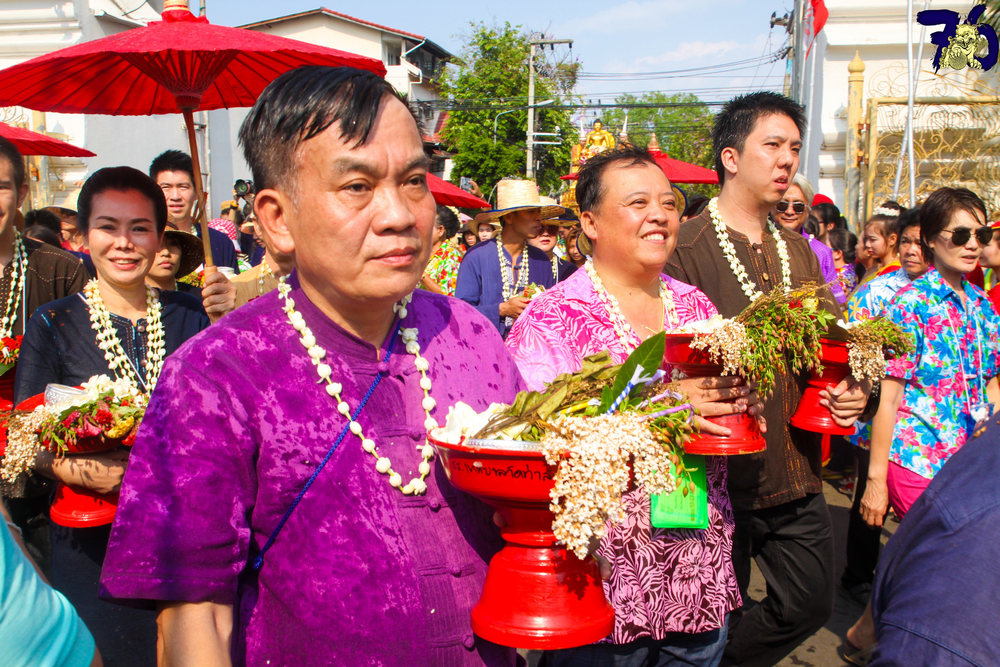
\includegraphics[scale=0.25]{../figures/image1/image_01.png}
    \caption{Imágen usada para generar el modelo.}
    \label{fig:imagen-entrenamiento}
\end{figure}
Primero se exporta la imágen y se selecciona un número arbitrario de pixeles, aunque lo que se guarda en memoria son los índices de esos pixeles de la imágen no su información RGB:
\begin{minted}[
    frame=none,
    autogobble,
    obeytabs=false,
    breaklines,
    tabsize=4,
    linenos=true,
    % numbersep=-10pt,
    baselinestretch=1,
    firstnumber=last,
    bgcolor=bg!70,
    ]{julia}
    julia> img_path = "../figures/image1/image_01.png";

    julia> img = sd.load(img_path);

    julia> rawind = sd.rawPixelIndexes(img);
    Select several pixels from skin and the background.
    Left-click for skin.
    Right-cligk for not-skin.
\end{minted}

Posterior a la selección de índices se hace un filtrado como se muestra en \code{filtind} para remover repetidos, se selecciona un número deseado de índices y posteriormente se usan esos índices para extraer la información de sus pixeles correspondientes guardados en la variable \code{pixels}. Cabe mencionar que el número de pixeles usado para generar el modelo fue de 15 en vez de 10.
\begin{minted}[
    frame=none,
    autogobble,
    obeytabs=false,
    breaklines,
    tabsize=4,
    linenos=true,
    mathescape,
    % numbersep=-10pt,
    baselinestretch=1,
    firstnumber=last,
    bgcolor=bg!70,
    ]{julia}
    julia> filtind = sd.filterPixelIndexes(rawind, 15);

    julia> pixels = sd.pixelSet(filtind, img);

    julia> μskin = sd.avgVector(pixels.skin); μbg = sd.avgVector(pixels.bg);

    julia> Σskin = sd.covarianceMatrix(pixels.skin, μskin); Σbg = sd.covarianceMatrix(pixels.bg, μbg);

    julia> lambda = 0.35; distskin, distbg, postskin, postbg = sd.probabilityDistributions(img, μskin, μbg, Σskin, Σbg, lambda); # compute probability distributions $\label{line:lambda}$
\end{minted}

Para calcular la probabilidad a priori de piel y no piel de la \cref{fig:imagen-entrenamiento} simplemente se tomó una estimación entre 0 y 1 para definir dicha probabilidad dependiendo de la cantitad de piel percibida en la imagen y usando una distribución de Bernoulli $\text{Bern}_{w}[\lambda]$, donde $\lambda$ corresponde a la probabilidad de observar el estado $w = 1$ el cual representa el caso de la piel,
\begin{equation*}
    Bern_{w}[\lambda] = 
    \begin{cases}
        \lambda & \text{si } w = 1 ,\\
        1 - \lambda & \text{si } w = 0 .
    \end{cases}
\end{equation*}
Para la \cref{fig:imagen-entrenamiento} se eligió un valor $\lambda = 0.35$ como se muestra en la línea \ref{line:lambda} donde también se computan las funciones Gaussianas tridimensionales tanto para la piel como para el fondo.

Los vectores promedio encontrados fueron (por simplicidad solamente se muestran los decimales hasta 5 cifras en todos los casos),
\begin{align*}
    \vec{\mu}_{\text{piel}} & =
    \begin{bmatrix}
        0.76575 \\
        0.49202 \\
        0.38666
    \end{bmatrix} , &
    \vec{\mu}_{\text{fondo}} & =
    \begin{bmatrix}
        0.50013 \\
        0.33202 \\
        0.35607 \\
    \end{bmatrix} .
\end{align*}
Las matrices de covarianza para ambos casos son,
\begin{align*}
    \Sigma_{\text{piel}} & = 
    \begin{bmatrix}
        0.04624 & 0.03660 & 0.03041 \\
        0.03660 & 0.03272 & 0.02909 \\
        0.03041 & 0.02909 & 0.02928
    \end{bmatrix} , &
    \Sigma_{\text{fondo}} & = 
    \begin{bmatrix}
        0.11992 & 0.02544 & 0.01760 \\
        0.02544 & 0.10546 & 0.10826 \\
        0.01760 & 0.10826 & 0.14839
    \end{bmatrix} .
\end{align*}
De donde se obtienen $\text{Pr}(x | w = 1)$ asociada a $\mu_{\text{piel}}$ y $\Sigma_{\text{piel}}$, y $\text{Pr}(x | w = 0)$ asociada a $\mu_{\text{fondo}}$ y $\Sigma_{\text{fondo}}$.

Después de calcular los vectores promedio y matrices de covarianza se procedió a computar los mapas logarítmicos de calor de la distribución aplicada a la imágen de entrenamiento mostrada en la \cref{fig:training} tanto para la piel, \cref{fig:training_distskin} como para lo no piel, \cref{fig:training_distbg}. En las \cref{fig:training_postskin,fig:training_postbg} se muestran los mapas de calor correspondientes de la probabilidad a posteriori $\text{Pr}(w | x^{\star})$ para piel y no piel, respectivamente.
\begin{figure}[h!]
    \centering
    \begin{subfigure}{0.4\textwidth}
        \centering
        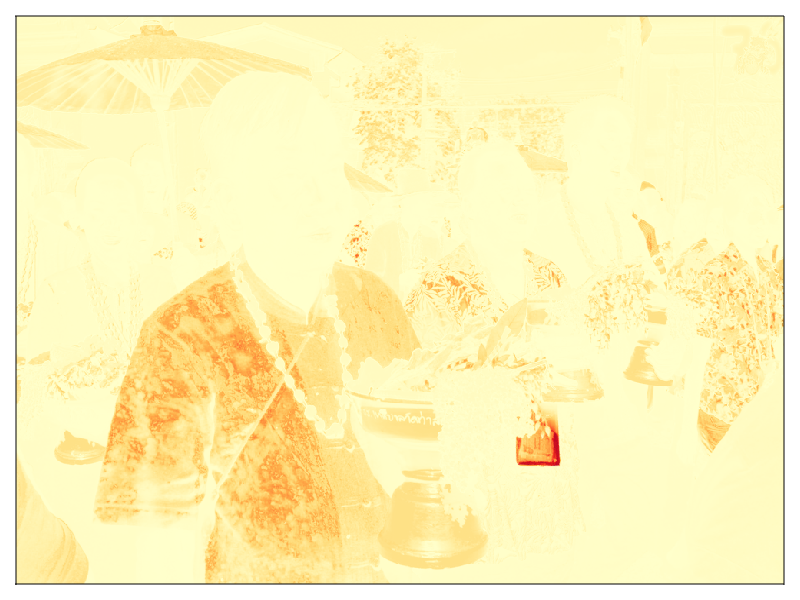
\includegraphics[width=\textwidth]{../figures/image1/image_01_distskin.png}
        \caption{Modelo de piel aplicado a la imagen de entrenamiento, $\log(\text{Pr}(x | w=1))$.}
        \label{fig:training_distskin}
    \end{subfigure}
    \hspace{1cm}
    %
    \begin{subfigure}{0.4\textwidth}
        \centering
        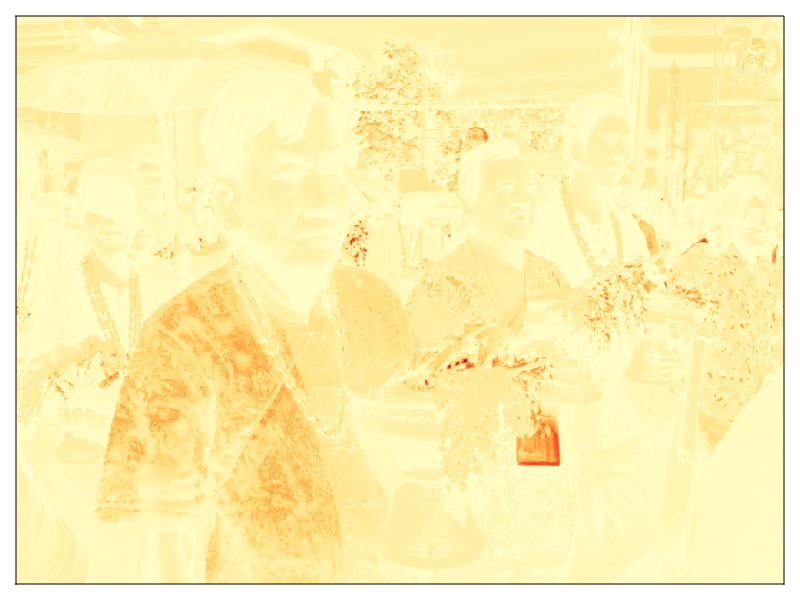
\includegraphics[width=\textwidth]{../figures/image1/image_01_distbg.png}
        \caption{Modelo de no piel aplicado a la imagen de entrenamiento, $\log(\text{Pr}(x | w=0))$.}
        \label{fig:training_distbg}
    \end{subfigure}
    %
    \begin{subfigure}{0.4\textwidth}
        \centering
        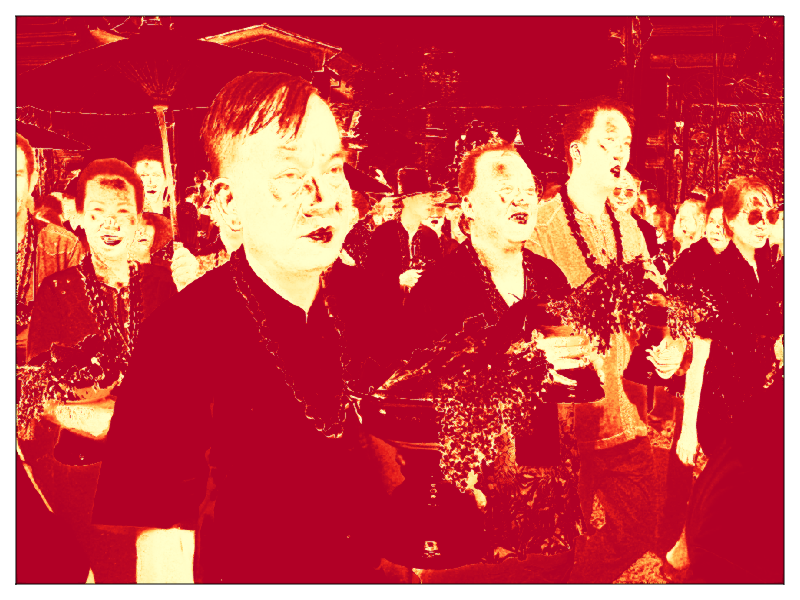
\includegraphics[width=\textwidth]{../figures/image1/image_01_postskin.png}
        \caption{Modelo a posteriori de piel aplicado a la imágen de entrenamiento, $\text{Pr}(w=1 | x^{\star})$.}
        \label{fig:training_postskin}
    \end{subfigure}
    \hspace{1cm}
    %
    \begin{subfigure}{0.4\textwidth}
        \centering
        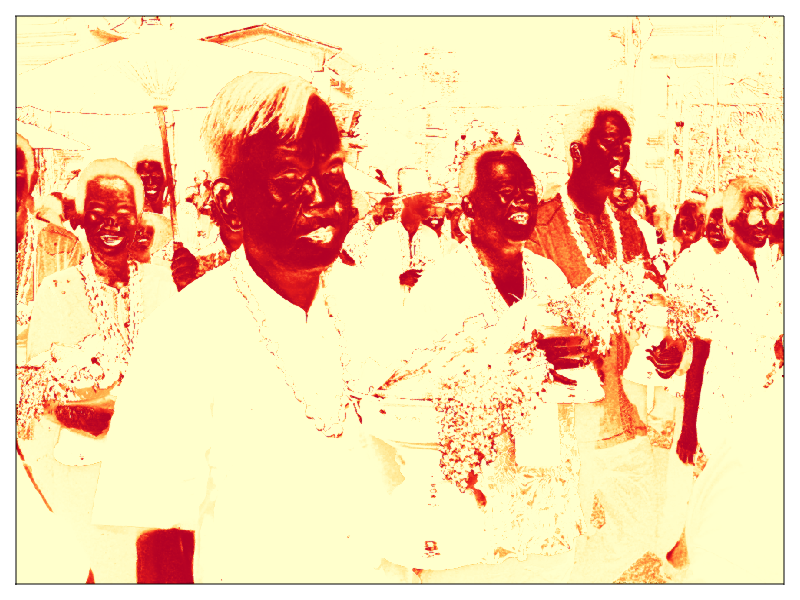
\includegraphics[width=\textwidth]{../figures/image1/image_01_postbg.png}
        \caption{Modelo a posteriori de no piel aplicado a la imágen de entrenamiento, $\text{Pr}(w=0 | x^{\star})$.}
        \label{fig:training_postbg}
    \end{subfigure}
    \caption{Mapas de calor del modelo para piel y no piel de la imágen de entrenamiento.}
    \label{fig:training}
\end{figure}

Los mapas de calor se obtienen como se muestra a continuación:
\begin{minted}[
    frame=none,
    autogobble,
    obeytabs=false,
    breaklines,
    tabsize=4,
    linenos=true,
    mathescape,
    % numbersep=-10pt,
    baselinestretch=1,
    firstnumber=last,
    bgcolor=bg!70,
    ]{julia}
    julia> distskinfig = sd.heatMap(log10.(distskin));

    julia> distbgfig = sd.heatMap(log10.(distbg));

    julia> postskinfig = sd.heatMap(postskin);

    julia> postbgfig = sd.heatMap(postbg);

    julia> tparam = 0.4; tresholdskin = map(x -> x > tparam ? x = 1 : x = 0, postskin); tresholdbg = map(x -> x > tparam ? x = 1 : x = 0, postbg);

    julia> treshskinfig = sd.heatMap(tresholdskin);

    julia> treshbgfig = sd.heatMap(tresholdbg);
\end{minted}

Donde \code{tparam} es el nombre de la variable del parámetro para hacer la clasificación binaria equivalente a $\text{T}$; las primeras dos instrucciones corresponden al computo del mapa de calor de la imagen respecto a sus Gaussianas iniciales, y el siguiente par de instrucciones son los mapas de calor respecto de sus distribuciones de probabilidad a posteriori. Posteriormente se computan las distribuciones binarias y sus respectivos mapas de calor para diferentes valores de $\text{T}$ como se muestra en la \cref{fig:binary_heatmaps_training}. Las instrucciones de código mostradas se repiten para todos los casos, el modelo se entrena partiendo desde el comienzo de las instrucciones y las pruebas del modelo a otras imágenes se realizan a partir de la línea \ref{line:lambda}, sólamente se tiene que importar la nueva imágen para ser utilizada.

No se logra ver una diferencia notable entre los diferentes valores del parámetro $\text{T}$, pero al observar detenidamente las caras de las personas en los mapas binarios correspondientes a la piel en las \cref{fig:training_treshskin_4,fig:training_treshskin_5,fig:training_treshskin_6} se observa el comienzo de la representación erronea de la clasificación de los pixeles. Mientras más aumenta $\text{T}$ más pixeles son erróneamente clasificados para este caso en particular aplicando el modelo a la propia imágen de entrenamiento. Aunque también se observa el efecto opuesto en que pixeles pertenecientes a elementos como ropa u objetos que se clasificaron como piel con $\text{T}=0.4$ cambian a no piel cuando $\text{T}=0.6$. La consecuencia observada es que el modelo binario resultante resulta más estricto al decidir si un pixel dado corresponde a piel o no al aumentar el valor de $\text{T}$.
\begin{figure}[ht!]
    \centering
    \begin{subfigure}{0.4\textwidth}
        \centering
        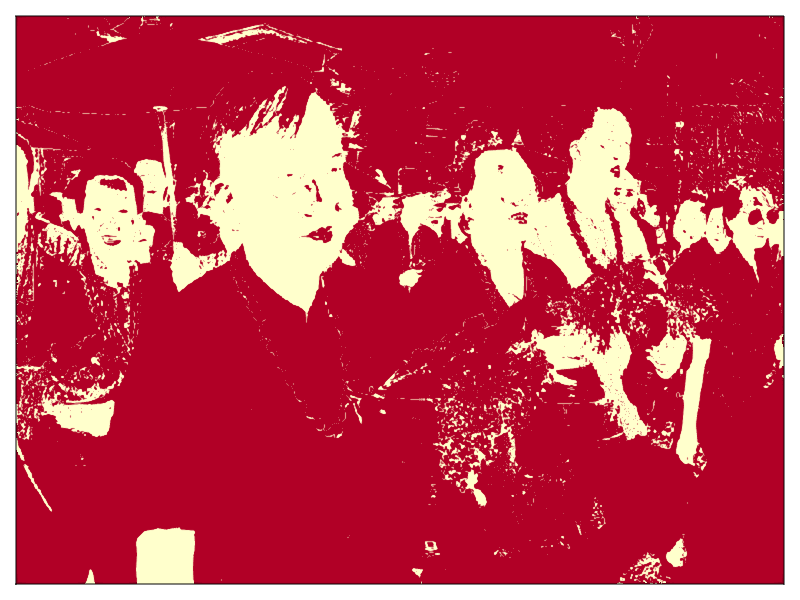
\includegraphics[width=\textwidth]{../figures/image1/image_01_treshskin_40percent.png}
        \caption{Piel; $\text{T} = 0.4$.}
        \label{fig:training_treshskin_4}
    \end{subfigure}
    \hspace{1cm}
    %
    \begin{subfigure}{0.4\textwidth}
        \centering
        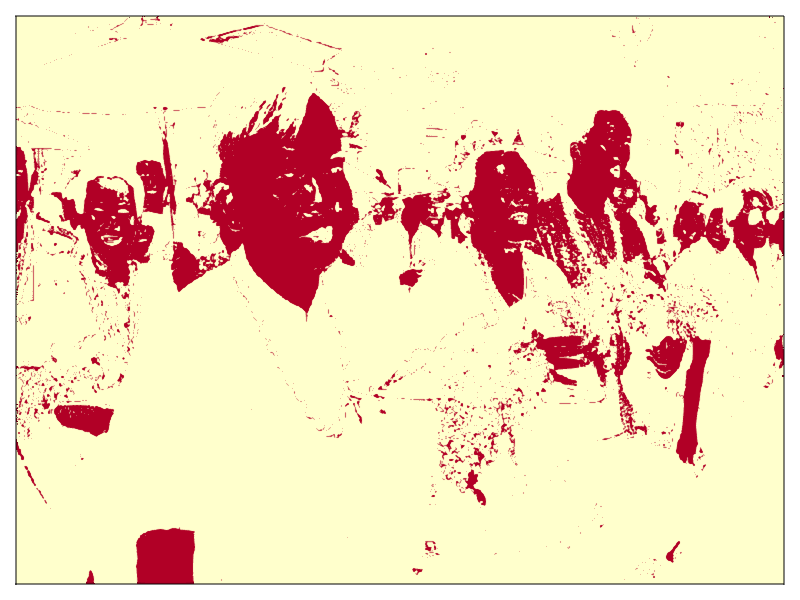
\includegraphics[width=\textwidth]{../figures/image1/image_01_treshbg_40percent.png}
        \caption{No piel; $\text{T} = 0.4$.}
        \label{fig:training_treshbg_4}
    \end{subfigure}
    %
    \begin{subfigure}{0.4\textwidth}
        \centering
        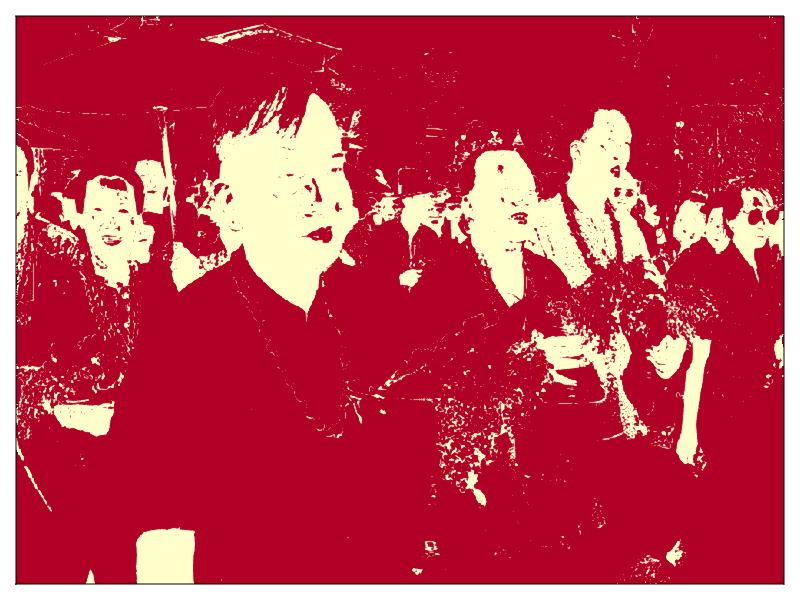
\includegraphics[width=\textwidth]{../figures/image1/image_01_treshskin_50percent.png}
        \caption{Piel; $\text{T} = 0.5$.}
        \label{fig:training_treshskin_5}
    \end{subfigure}
    \hspace{1cm}
    %
    \begin{subfigure}{0.4\textwidth}
        \centering
        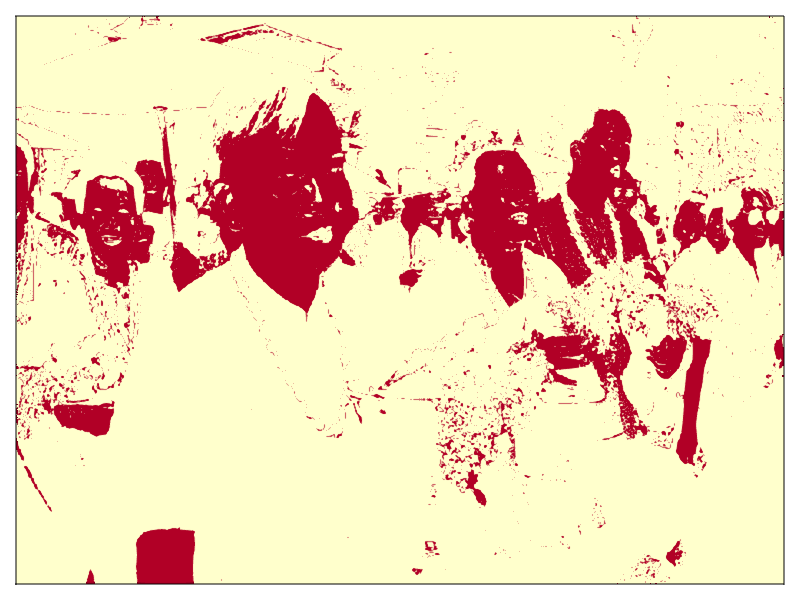
\includegraphics[width=\textwidth]{../figures/image1/image_01_treshbg_50percent.png}
        \caption{No piel; $\text{T} = 0.5$.}
        \label{fig:training_treshbg_5}
    \end{subfigure}
    %
    \begin{subfigure}{0.4\textwidth}
        \centering
        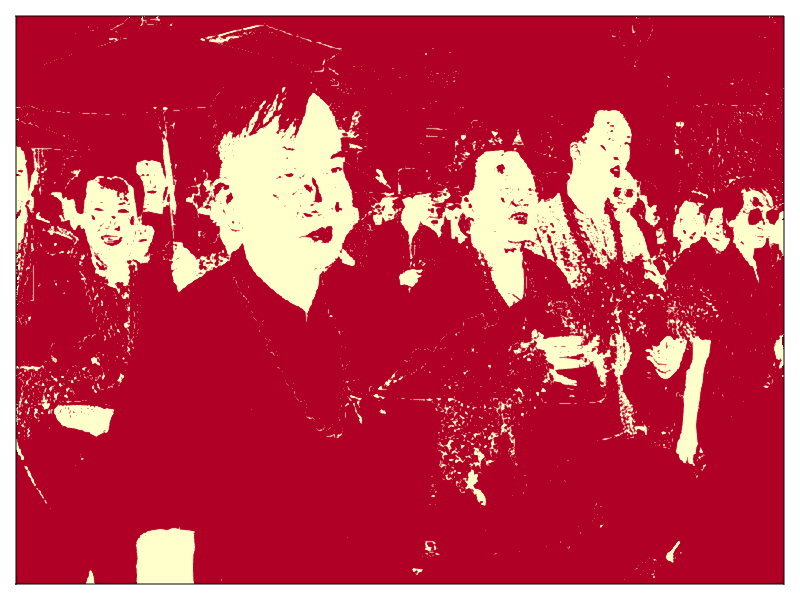
\includegraphics[width=\textwidth]{../figures/image1/image_01_treshskin_60percent.png}
        \caption{Piel; $\text{T} = 0.6$.}
        \label{fig:training_treshskin_6}
    \end{subfigure}
    \hspace{1cm}
    %
    \begin{subfigure}{0.4\textwidth}
        \centering
        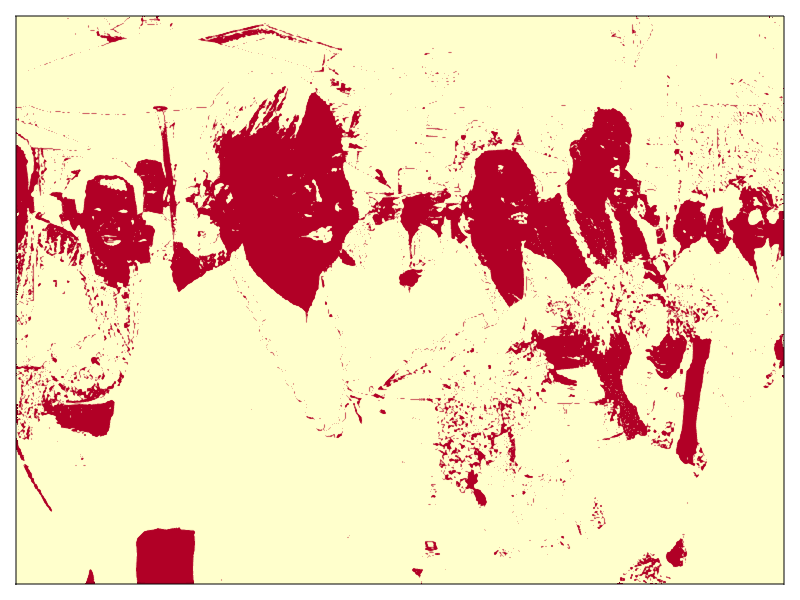
\includegraphics[width=\textwidth]{../figures/image1/image_01_treshbg_60percent.png}
        \caption{No piel; $\text{T} = 0.6$.}
        \label{fig:training_treshbg_6}
    \end{subfigure}
    \caption{Mapas de calor binarios.}
    \label{fig:binary_heatmaps_training}
\end{figure}

Este modelo se aplicó a las \cref{fig:imagen_prueba_no3,fig:imagen_prueba_no6,fig:imagen_prueba_no2}, y las imágenes resultantes de la aplicación del modelo se muestran en las \cref{fig:model_applied_no3,fig:model_applied_no6,fig:model_applied_no2}. Cabe mencionar que para cada una de ellas se eligió un valor de $\lambda$ para la probabilidad a priori que aproximara la cantidad observada de piel.
\begin{figure}[ht!]
    \centering
    \begin{subfigure}[t]{0.4\textwidth}
        \centering
        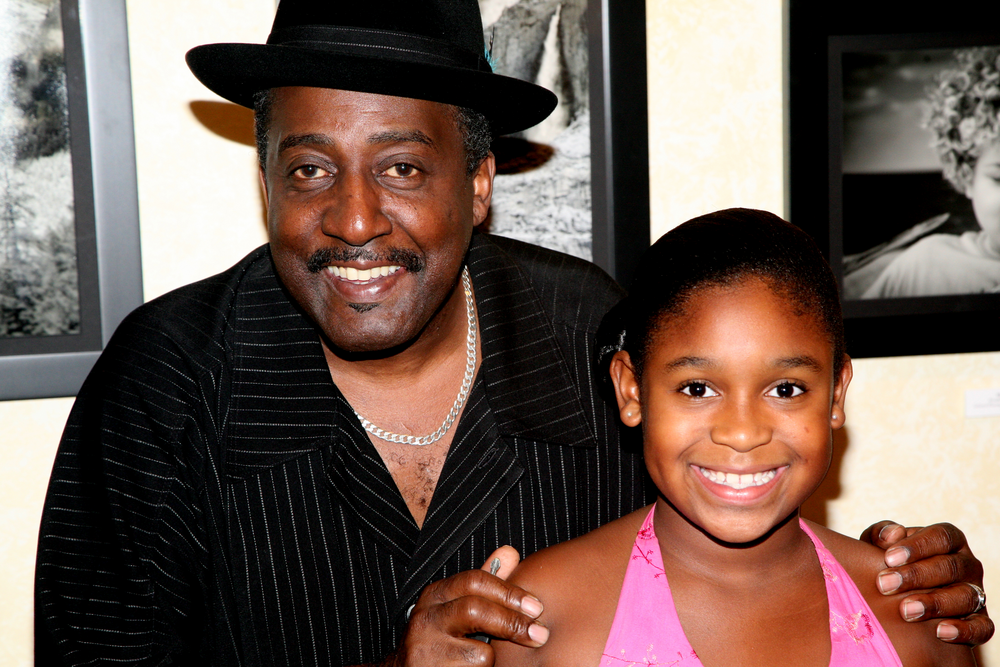
\includegraphics[width=\textwidth]{../figures/image3/image_03.png}
        \caption{Imágen de prueba con fondo semi homogeneo y en contraste con los tonos de piel.}
        \label{fig:imagen_prueba_no3}
    \end{subfigure}
    \hspace{1cm}
    %
    \begin{subfigure}[t]{0.4\textwidth}
        \centering
        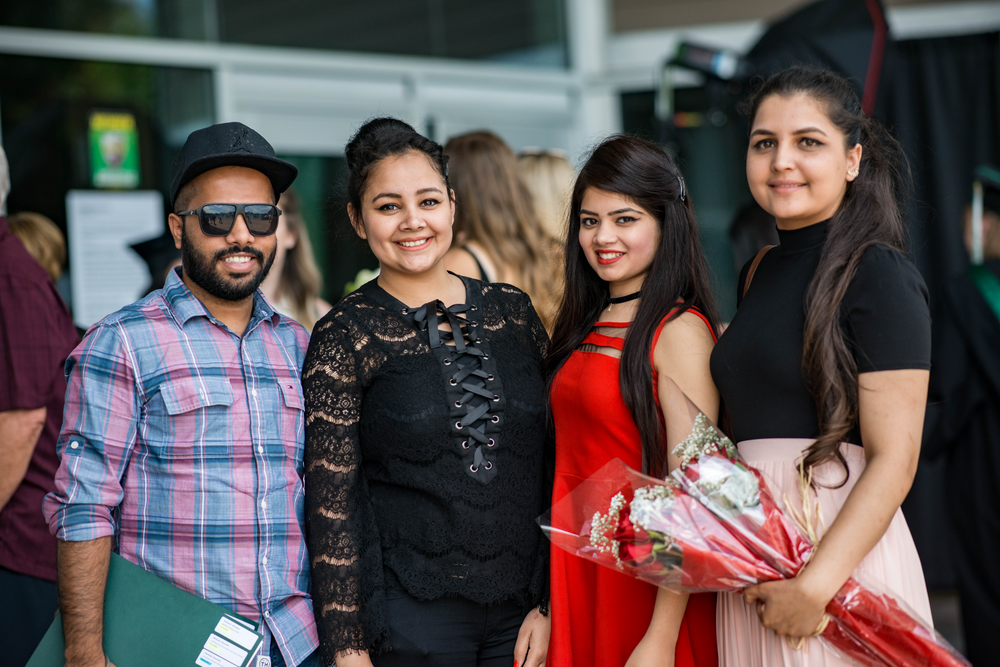
\includegraphics[width=\textwidth]{../figures/image6/image_06.png}
        \caption{Imágen de prueba con fondo variable.}
        \label{fig:imagen_prueba_no6}
        % \label{fig:training_postskin}
    \end{subfigure}
    %
    \begin{subfigure}{0.4\textwidth}
        \centering
        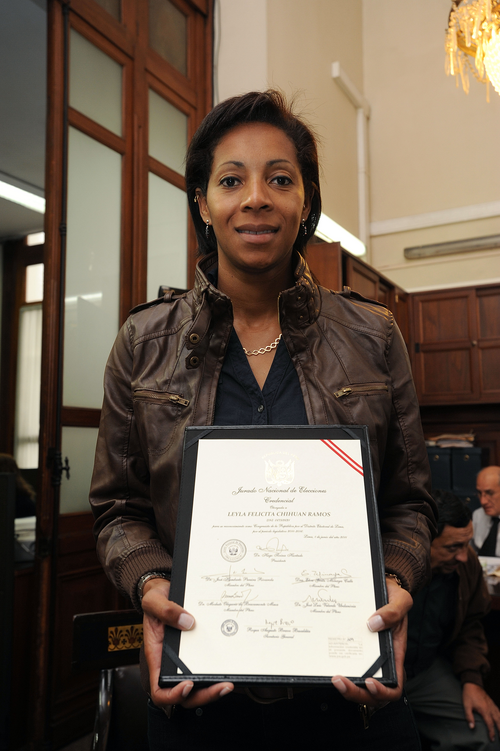
\includegraphics[width=0.7\textwidth]{../figures/image2/image_02.png}
        \caption{Imágen de prueba con tonos de fondo y piel similares.}
        \label{fig:imagen_prueba_no2}
        % \label{fig:training_distskin}
    \end{subfigure}
    %
    \caption{Imágenes elegidas para aplicar el modelo generado para la detección de piel.}
    % \label{fig:model_applied_no3}
\end{figure}

En la \cref{fig:imagen_prueba_no2} para el caso de la \cref{fig:model_applied_no2} hay un claro problema en la clasificación, tanto para la piel como para lo no piel. Se logra apreciar como partes de la puerta son mal clasificadas como piel como también sucede con los muebles de madera mostrados al fondo a la derecha de la persona en el centro de la imágen. Además, la clasificación binaria para esta imágen no parece mejorar notoriamente la mala representación de los pixeles de la puerta.

Algo similar sucede para el caso de la \cref{fig:imagen_prueba_no3}, donde la aplicación del modelo a ésta se muestra en la \cref{fig:model_applied_no3}, se obverva que la sombra que se produce por el sombrero del individuo vestido con camisa negra se mal clasifica originalmente como piel al usar la distribución de probabilidad a posteriori pero se mejora cuando se realiza la clasificación binaria.

Finalmente, para el caso de la \cref{fig:imagen_prueba_no6} todo parece clasificarse de manera correcta en la clasificación binaria. Aunque se puede observar pixeles mal clasificados alrededor del racimo de flores que aparece en la parte inferior derecha.

\newpage
\begin{figure}[ht!]
    \centering
    \begin{subfigure}{0.4\textwidth}
        \centering
        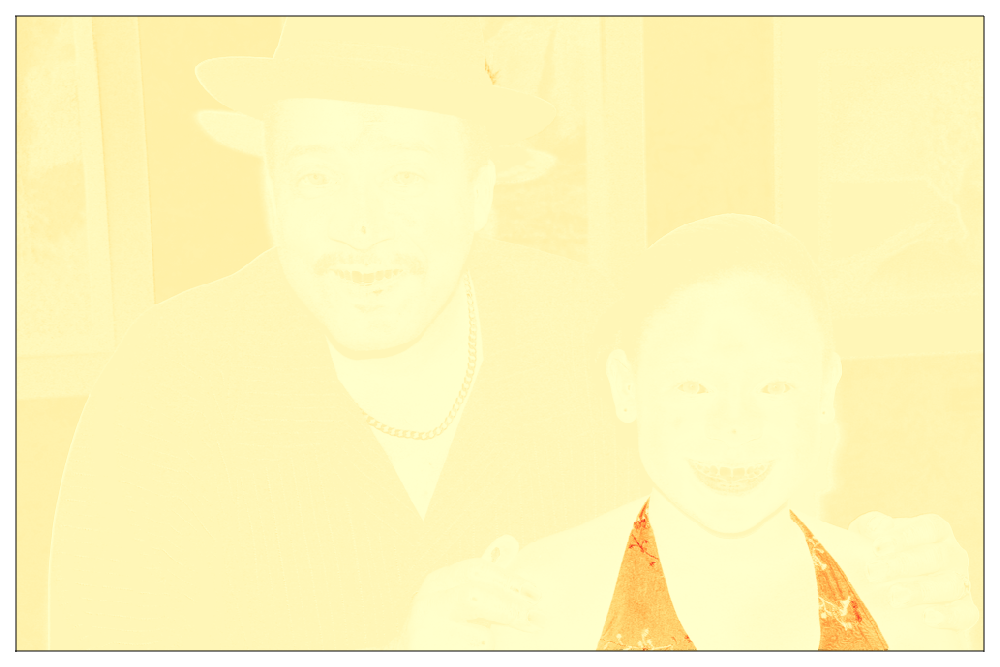
\includegraphics[width=0.8\textwidth]{../figures/image3/image_03_distskin.png}
        \caption{Modelo de piel, $\log(\text{Pr}(x | w=1))$.}
        % \label{fig:training_distskin}
    \end{subfigure}
    \hspace{1cm}
    %
    \begin{subfigure}{0.4\textwidth}
        \centering
        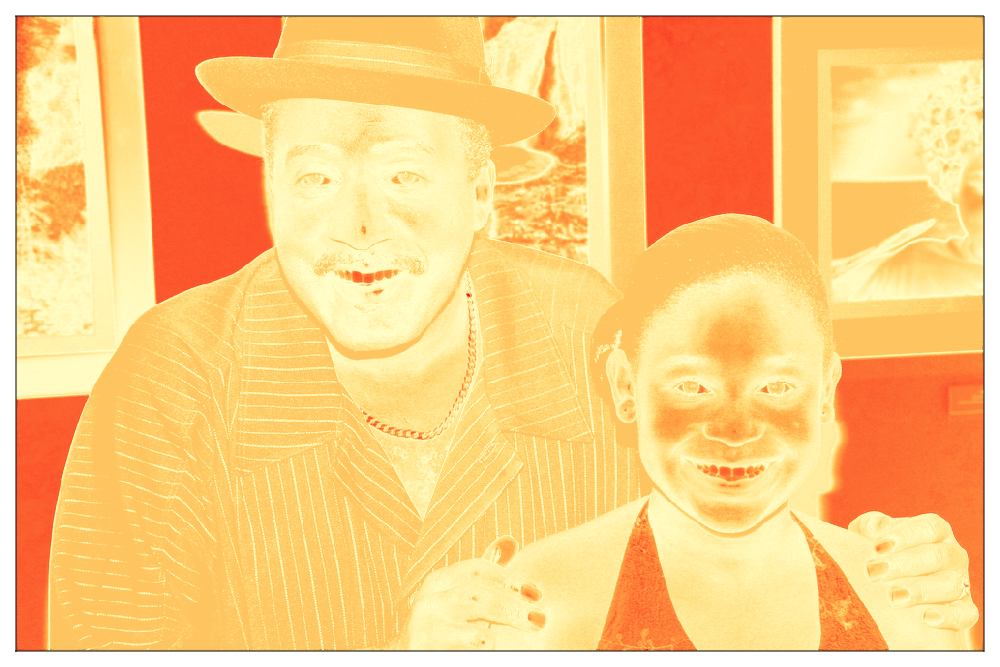
\includegraphics[width=0.8\textwidth]{../figures/image3/image_03_distbg.png}
        \caption{Modelo de no piel, $\log(\text{Pr}(x | w=0))$.}
        % \label{fig:training_distbg}
    \end{subfigure}
    %
    \begin{subfigure}{0.4\textwidth}
        \centering
        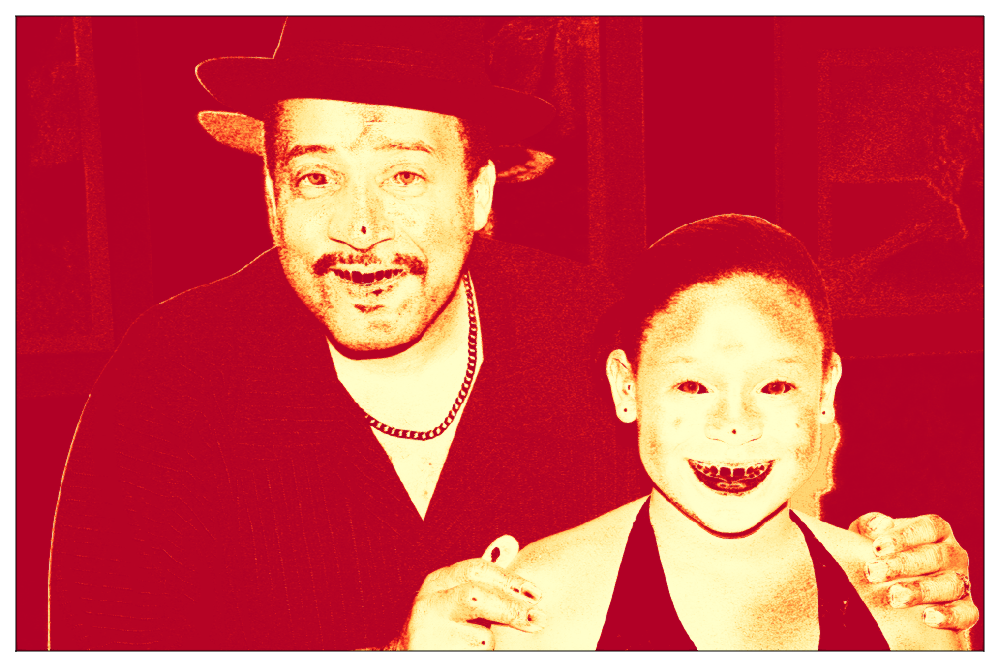
\includegraphics[width=0.8\textwidth]{../figures/image3/image_03_postskin.png}
        \caption{Modelo a posteriori de piel, $\text{Pr}(w=1 | x^{\star})$.}
        % \label{fig:training_postskin}
    \end{subfigure}
    \hspace{1cm}
    %
    \begin{subfigure}{0.4\textwidth}
        \centering
        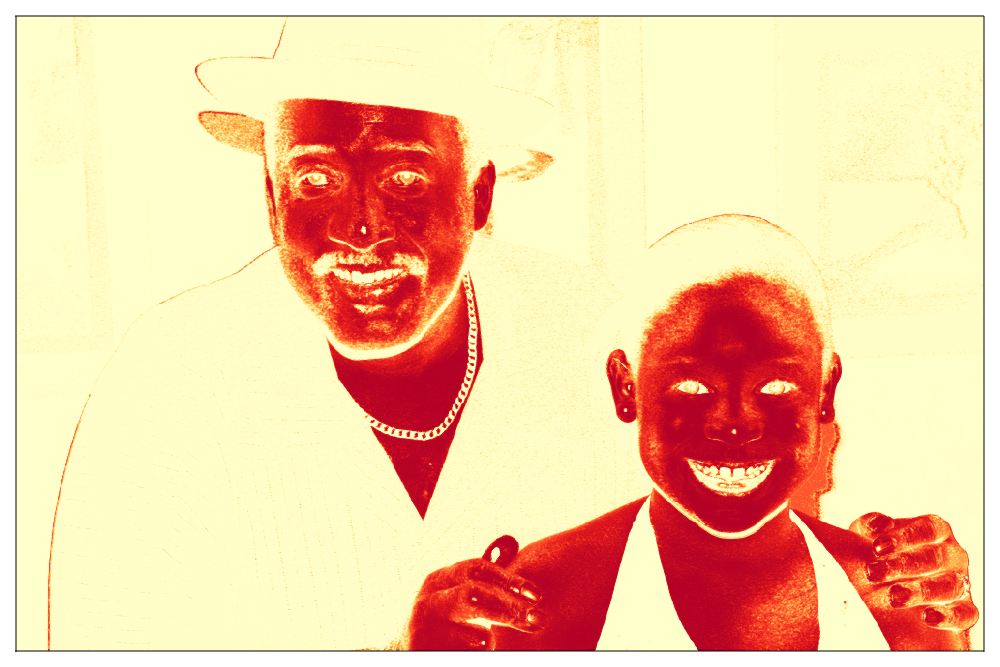
\includegraphics[width=0.8\textwidth]{../figures/image3/image_03_postbg.png}
        \caption{Modelo a posteriori de no piel, $\text{Pr}(w=0 | x^{\star})$.}
        % \label{fig:training_postbg}
    \end{subfigure}
    %
    \begin{subfigure}{0.4\textwidth}
        \centering
        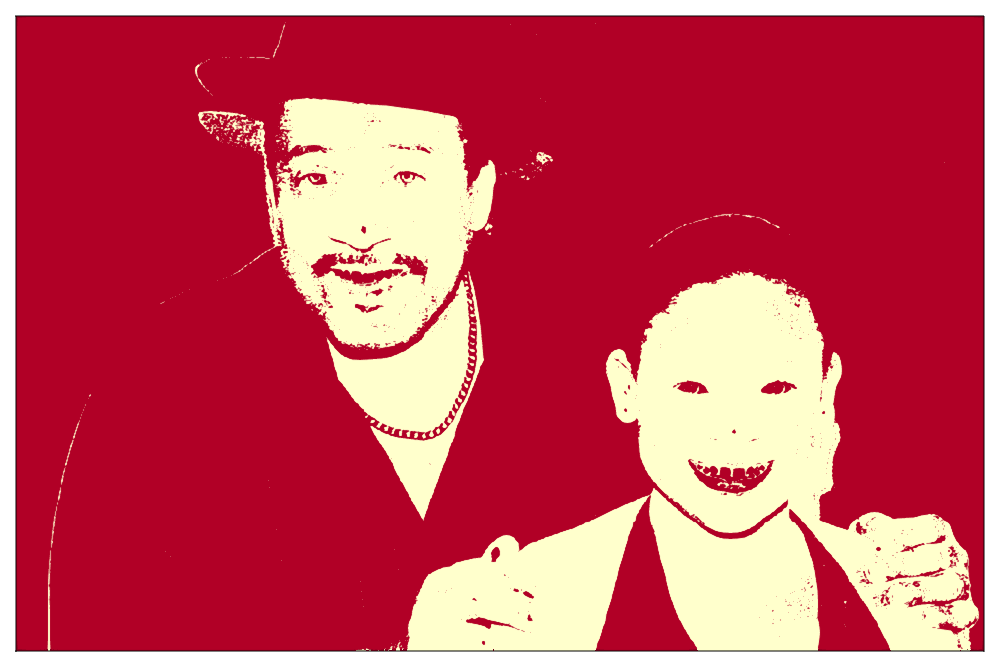
\includegraphics[width=0.8\textwidth]{../figures/image3/image_03_treshskin_40percent.png}
        \caption{Piel; $\text{T} = 0.4$.}
        % \label{fig:training_treshskin_4}
    \end{subfigure}
    \hspace{1cm}
    %
    \begin{subfigure}{0.4\textwidth}
        \centering
        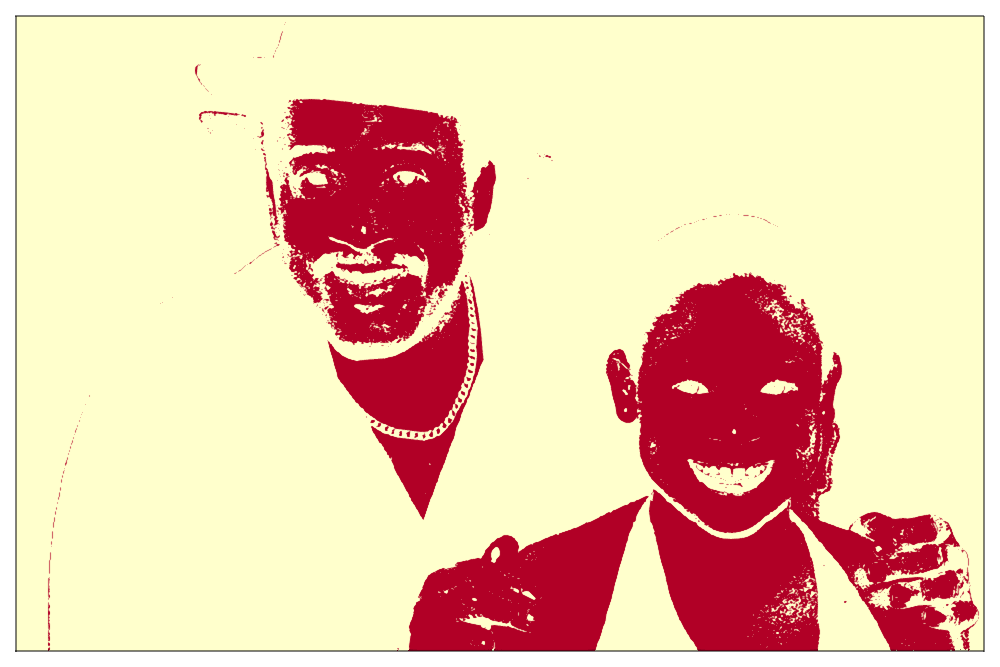
\includegraphics[width=0.8\textwidth]{../figures/image3/image_03_treshbg_40percent.png}
        \caption{No piel; $\text{T} = 0.4$.}
        % \label{fig:training_treshbg_4}
    \end{subfigure}
    %
    \begin{subfigure}{0.4\textwidth}
        \centering
        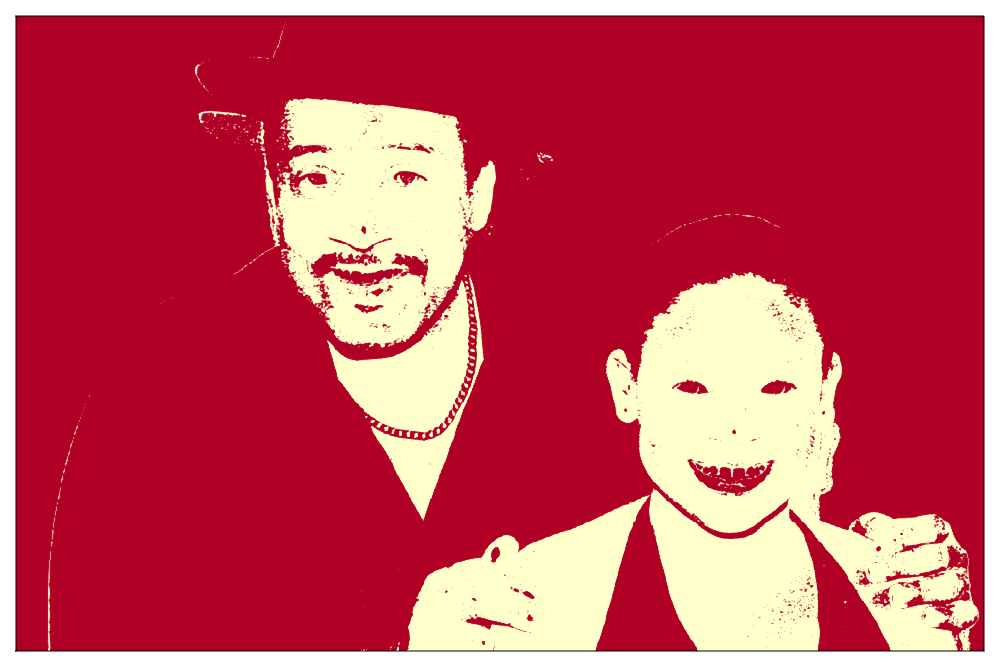
\includegraphics[width=0.8\textwidth]{../figures/image3/image_03_treshskin_50percent.png}
        \caption{Piel; $\text{T} = 0.5$.}
        % \label{fig:training_treshskin_5}
    \end{subfigure}
    \hspace{1cm}
    %
    \begin{subfigure}{0.4\textwidth}
        \centering
        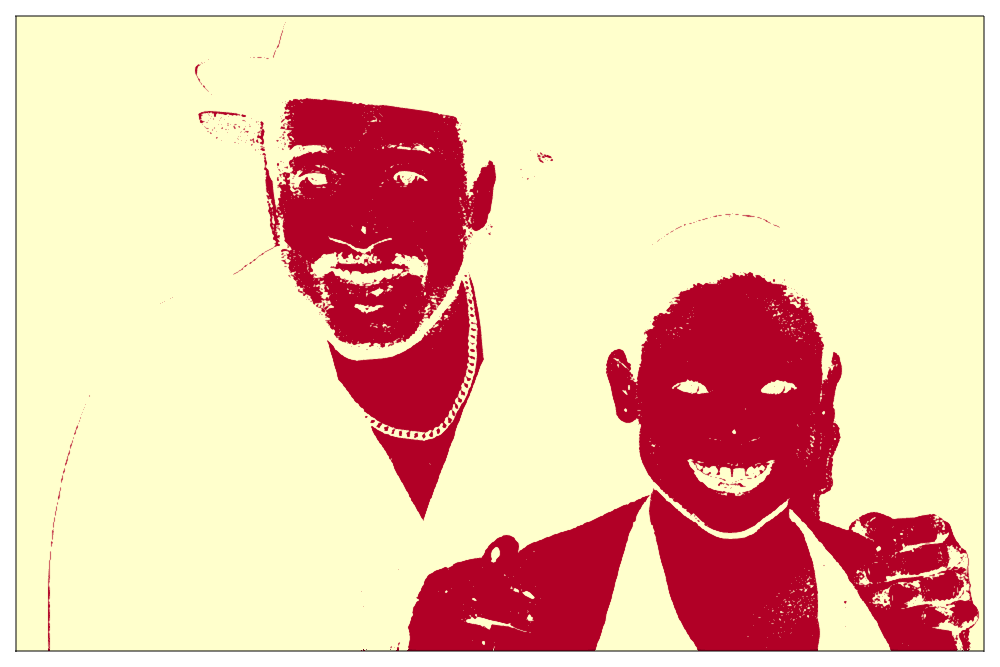
\includegraphics[width=0.8\textwidth]{../figures/image3/image_03_treshbg_50percent.png}
        \caption{No piel; $\text{T} = 0.5$.}
        % \label{fig:training_treshbg_5}
    \end{subfigure}
    %
    \begin{subfigure}{0.4\textwidth}
        \centering
        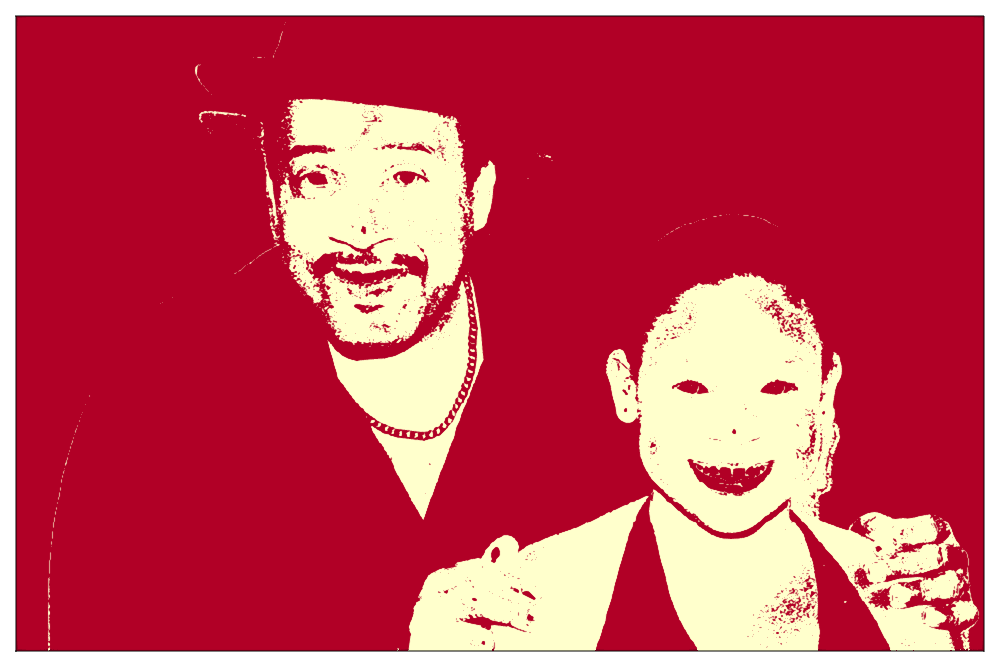
\includegraphics[width=0.8\textwidth]{../figures/image3/image_03_treshskin_60percent.png}
        \caption{Piel; $\text{T} = 0.6$.}
        % \label{fig:training_treshskin_6}
    \end{subfigure}
    \hspace{1cm}
    %
    \begin{subfigure}{0.4\textwidth}
        \centering
        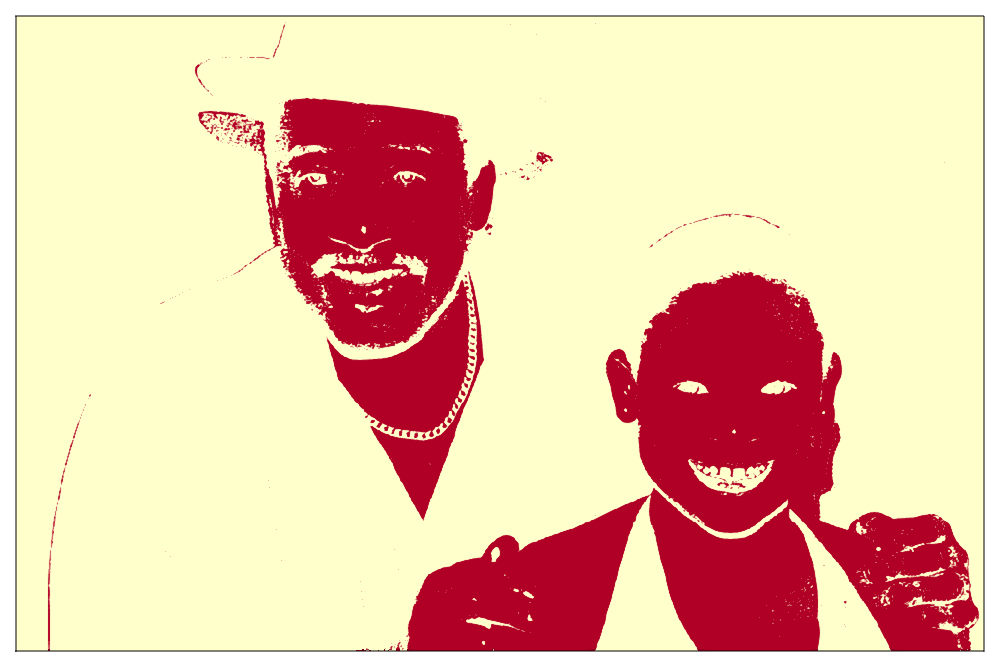
\includegraphics[width=0.8\textwidth]{../figures/image3/image_03_treshbg_60percent.png}
        \caption{No piel; $\text{T} = 0.6$.}
        % \label{fig:training_treshbg_6}
    \end{subfigure}
    \caption{Mapas de calor del modelo para piel y no piel de la imágen \cref{fig:imagen_prueba_no3}.}
    \label{fig:model_applied_no3}
\end{figure}

\newpage
\begin{figure}[ht!]
    \centering
    \begin{subfigure}{0.4\textwidth}
        \centering
        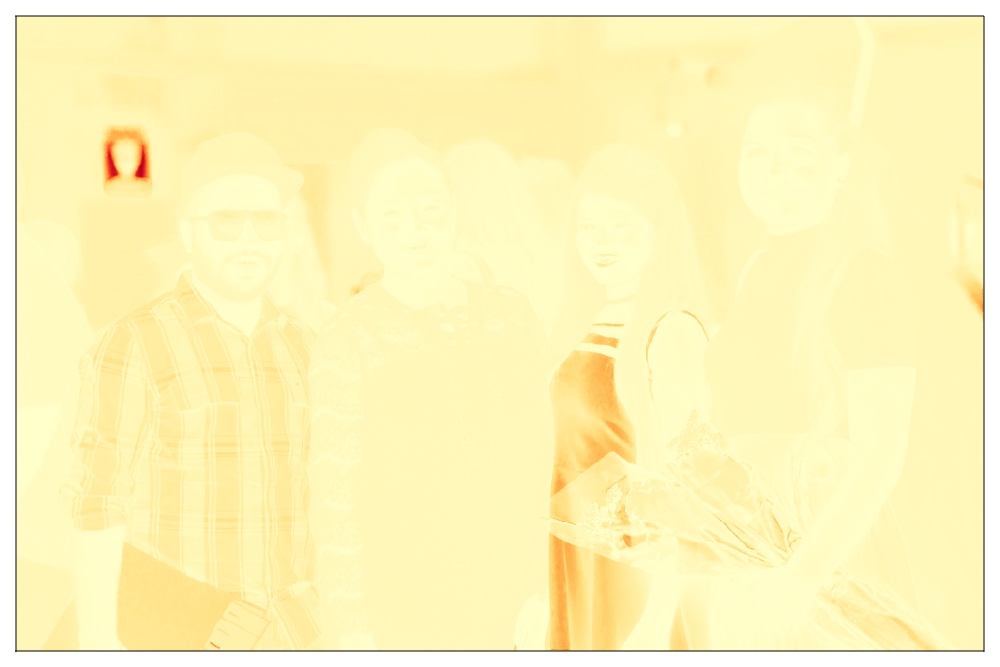
\includegraphics[width=0.8\textwidth]{../figures/image6/image_06_distskin.png}
        \caption{Modelo de piel, $\log(\text{Pr}(x | w=1))$.}
        % \label{fig:training_distskin}
    \end{subfigure}
    \hspace{1cm}
    %
    \begin{subfigure}{0.4\textwidth}
        \centering
        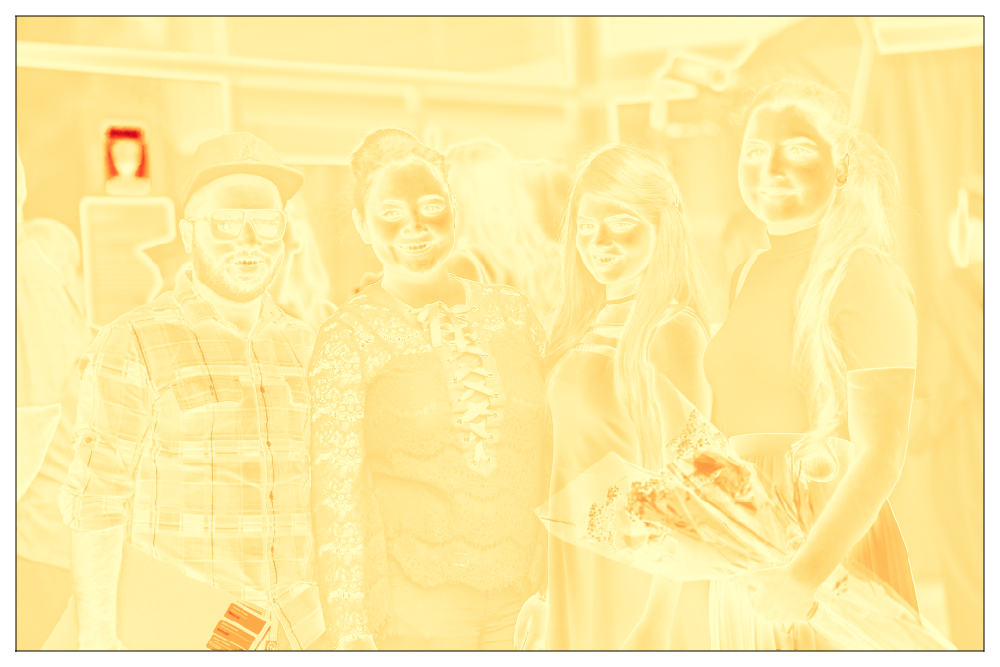
\includegraphics[width=0.8\textwidth]{../figures/image6/image_06_distbg.png}
        \caption{Modelo de no piel, $\log(\text{Pr}(x | w=0))$.}
        % \label{fig:training_distbg}
    \end{subfigure}
    %
    \begin{subfigure}{0.4\textwidth}
        \centering
        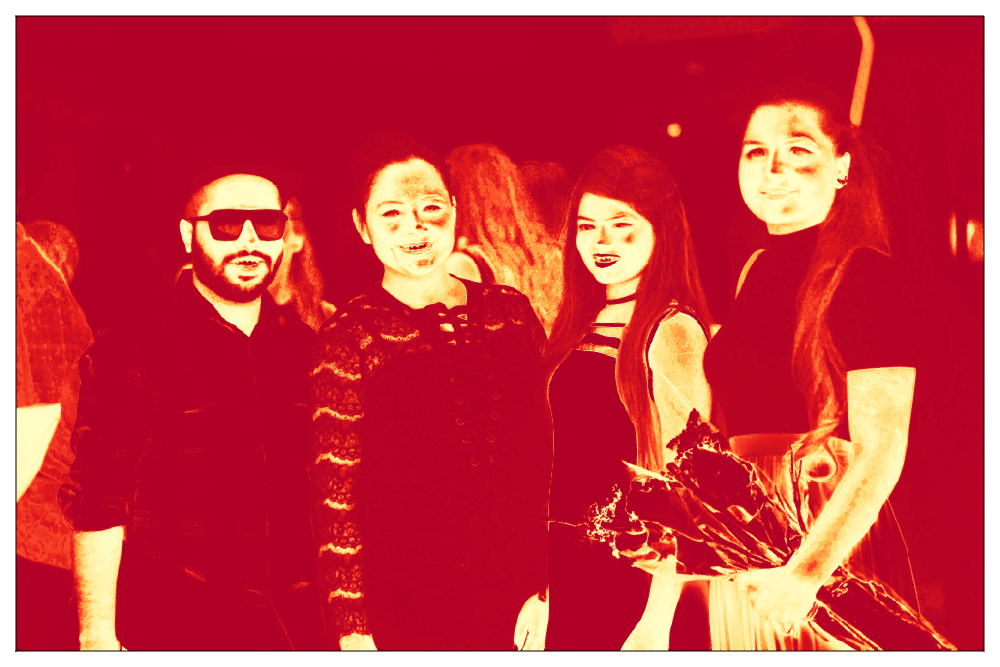
\includegraphics[width=0.8\textwidth]{../figures/image6/image_06_postskin.png}
        \caption{Modelo a posteriori de piel, $\text{Pr}(w=1 | x^{\star})$.}
        % \label{fig:training_postskin}
    \end{subfigure}
    \hspace{1cm}
    %
    \begin{subfigure}{0.4\textwidth}
        \centering
        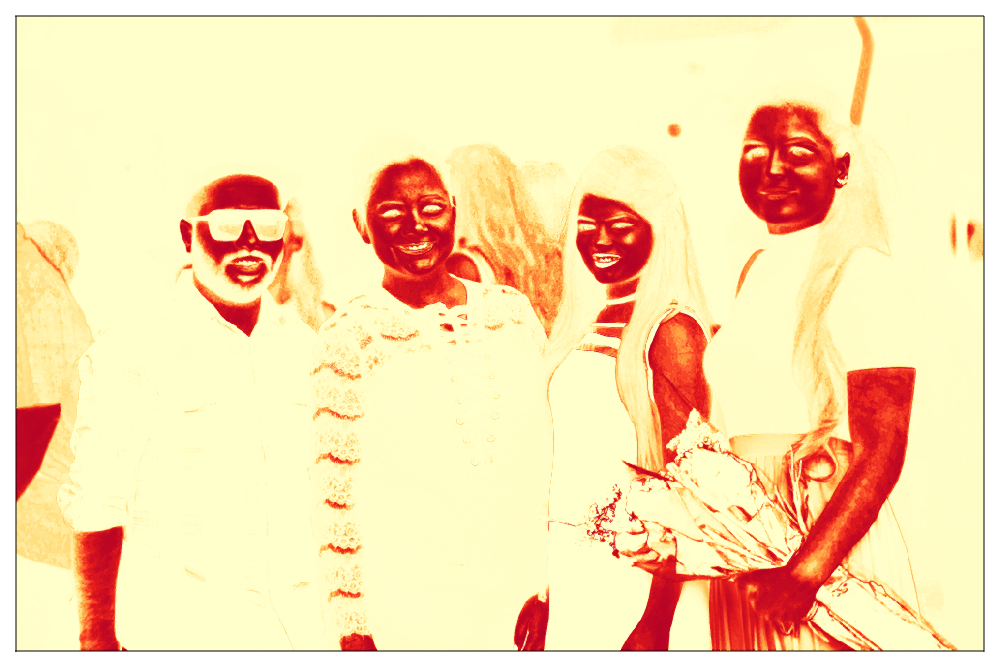
\includegraphics[width=0.8\textwidth]{../figures/image6/image_06_postbg.png}
        \caption{Modelo a posteriori de no piel, $\text{Pr}(w=0 | x^{\star})$.}
        % \label{fig:training_postbg}
    \end{subfigure}
    %
    \begin{subfigure}{0.4\textwidth}
        \centering
        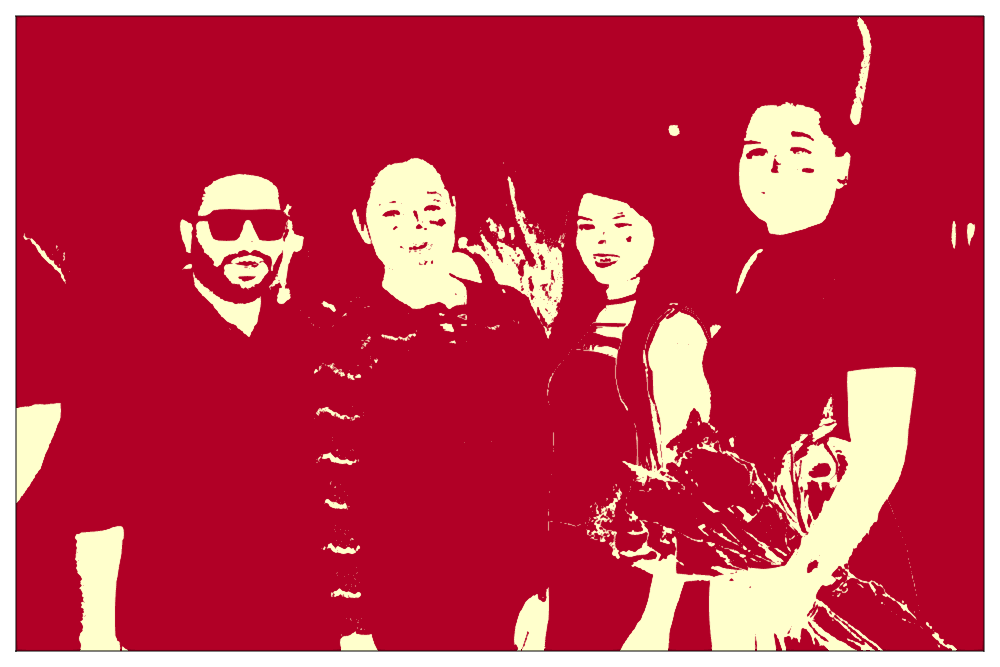
\includegraphics[width=0.8\textwidth]{../figures/image6/image_06_treshskin_40percent.png}
        \caption{Piel; $\text{T} = 0.4$.}
        % \label{fig:training_treshskin_4}
    \end{subfigure}
    \hspace{1cm}
    %
    \begin{subfigure}{0.4\textwidth}
        \centering
        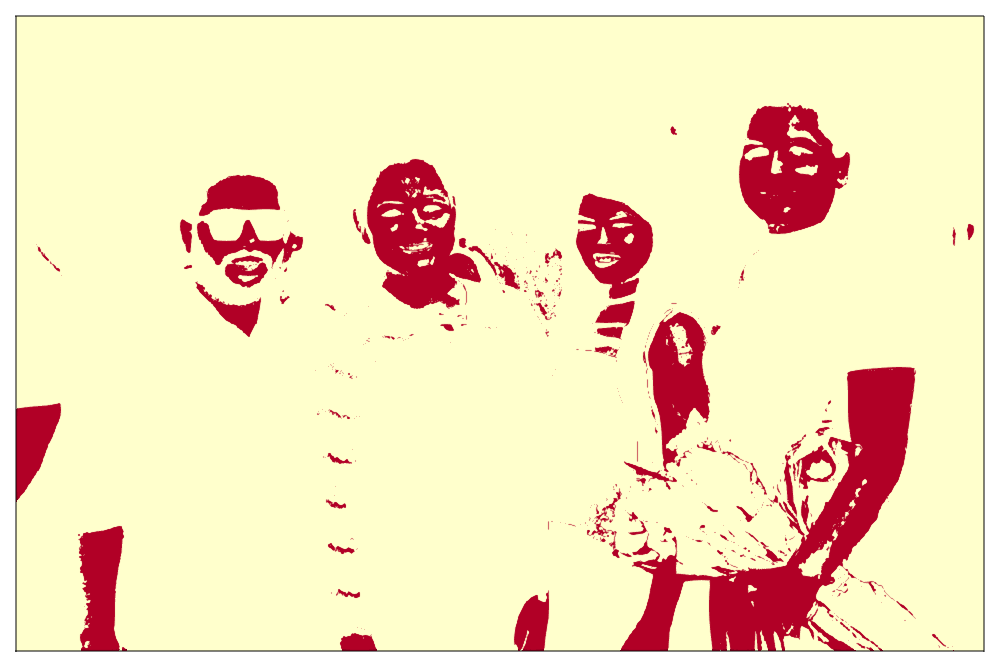
\includegraphics[width=0.8\textwidth]{../figures/image6/image_06_treshbg_40percent.png}
        \caption{No piel; $\text{T} = 0.4$.}
        % \label{fig:training_treshbg_4}
    \end{subfigure}
    %
    \begin{subfigure}{0.4\textwidth}
        \centering
        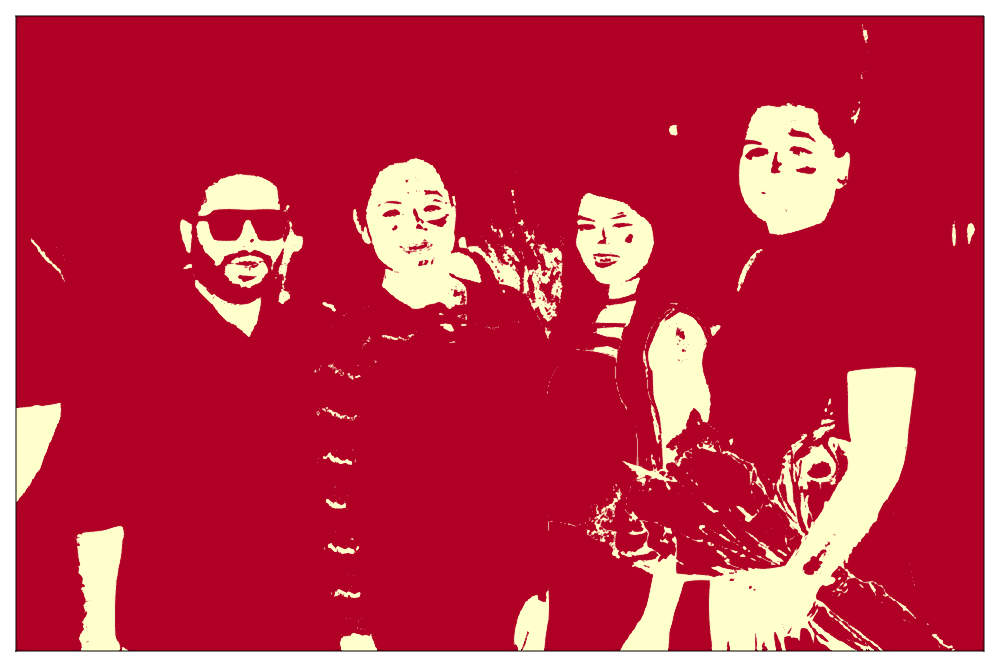
\includegraphics[width=0.8\textwidth]{../figures/image6/image_06_treshskin_50percent.png}
        \caption{Piel; $\text{T} = 0.5$.}
        % \label{fig:training_treshskin_5}
    \end{subfigure}
    \hspace{1cm}
    %
    \begin{subfigure}{0.4\textwidth}
        \centering
        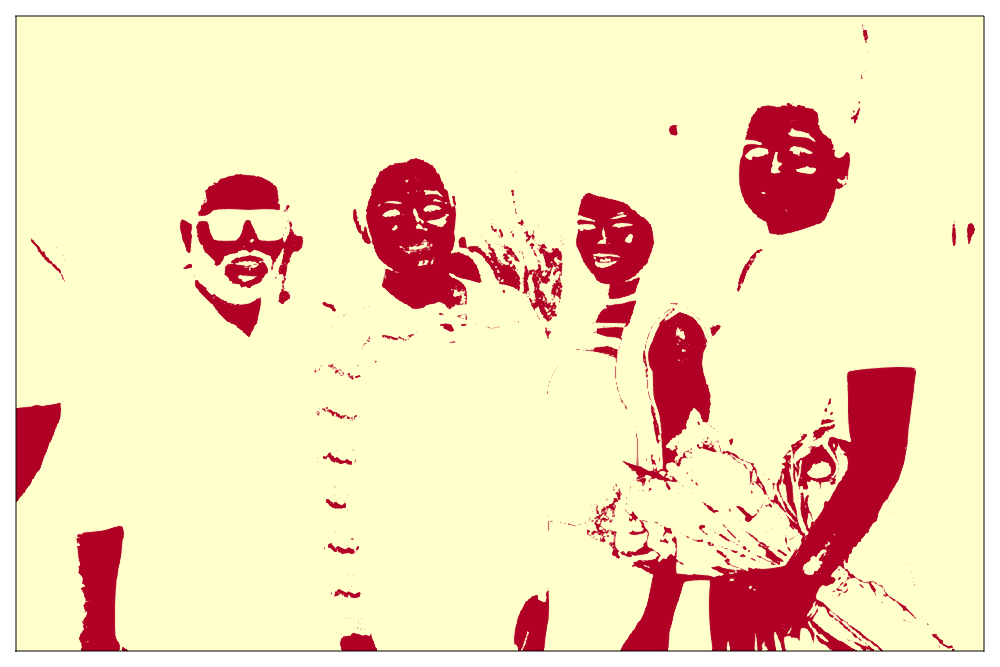
\includegraphics[width=0.8\textwidth]{../figures/image6/image_06_treshbg_50percent.png}
        \caption{No piel; $\text{T} = 0.5$.}
        % \label{fig:training_treshbg_5}
    \end{subfigure}
    %
    \begin{subfigure}{0.4\textwidth}
        \centering
        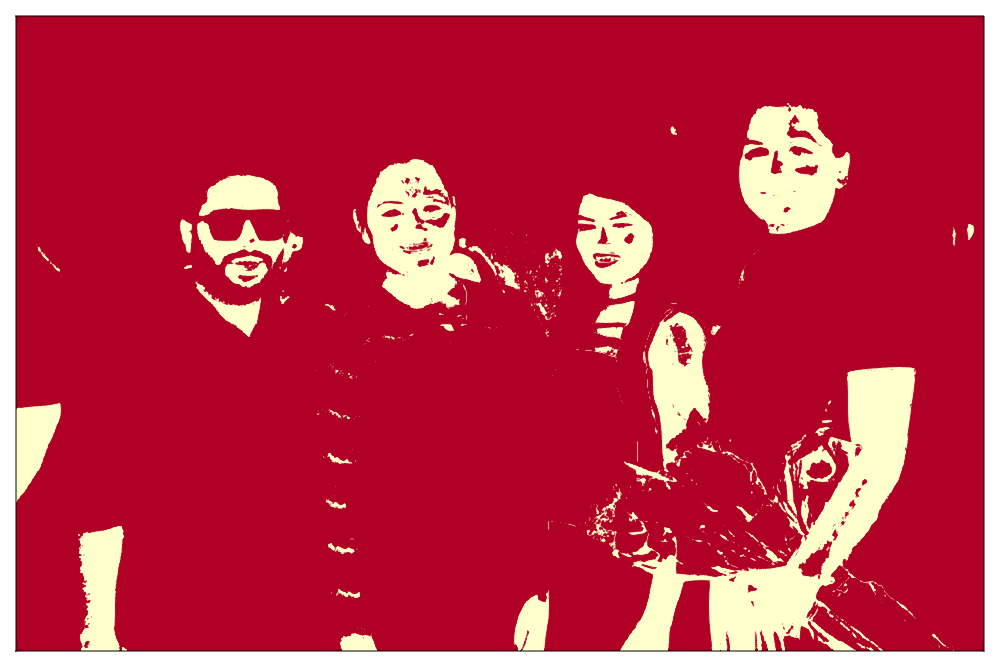
\includegraphics[width=0.8\textwidth]{../figures/image6/image_06_treshskin_60percent.png}
        \caption{Piel; $\text{T} = 0.6$.}
        % \label{fig:training_treshskin_6}
    \end{subfigure}
    \hspace{1cm}
    %
    \begin{subfigure}{0.4\textwidth}
        \centering
        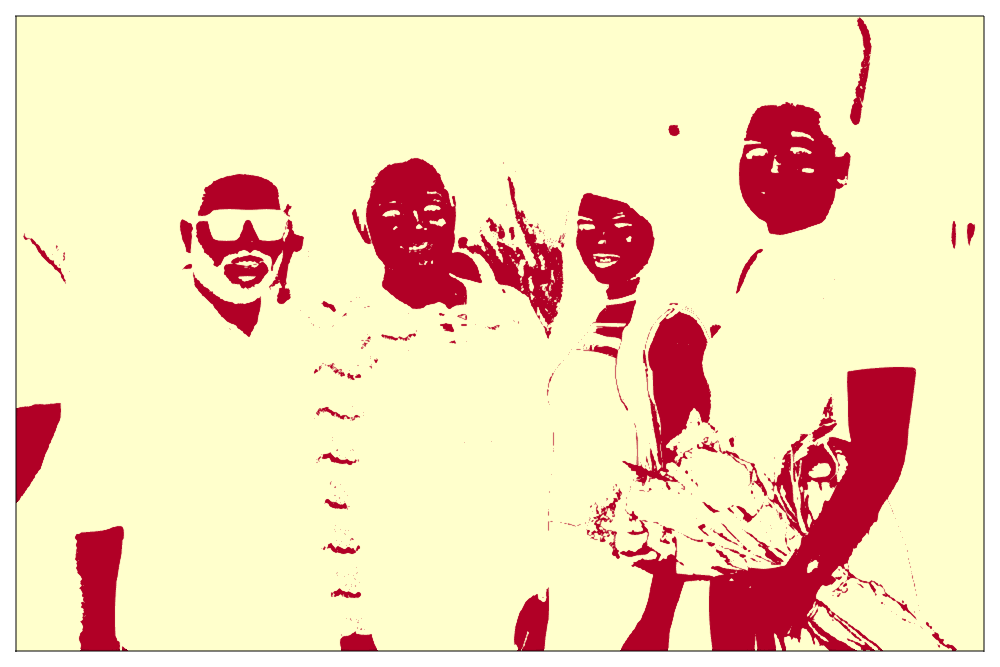
\includegraphics[width=0.8\textwidth]{../figures/image6/image_06_treshbg_60percent.png}
        \caption{No piel; $\text{T} = 0.6$.}
        % \label{fig:training_treshbg_6}
    \end{subfigure}
    \caption{Mapas de calor del modelo para piel y no piel de la imágen \cref{fig:imagen_prueba_no6}.}
    \label{fig:model_applied_no6}
\end{figure}

\newpage
\begin{figure}[ht!]
    \centering
    \begin{subfigure}[t]{0.2\textwidth}
        \centering
        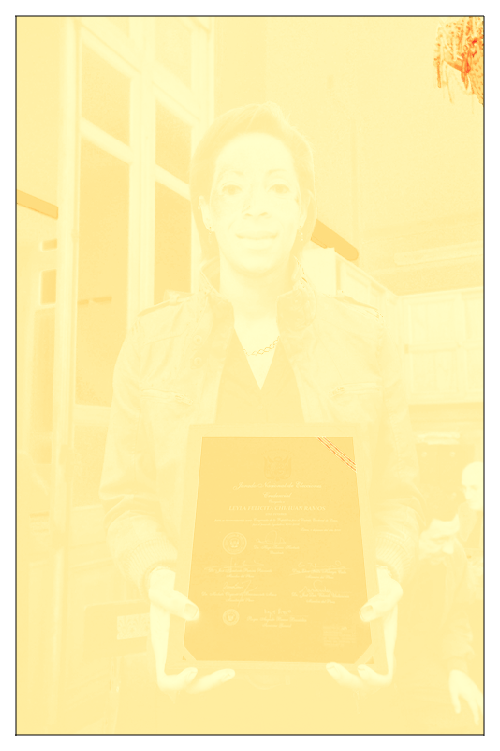
\includegraphics[width=\textwidth]{../figures/image2/image_02_distskin.png}
        \caption{Modelo de piel, $\log(\text{Pr}(x | w=1))$.}
        % \label{fig:training_distskin}
    \end{subfigure}
    \hspace{0.25cm}
    %
    \begin{subfigure}[t]{0.2\textwidth}
        \centering
        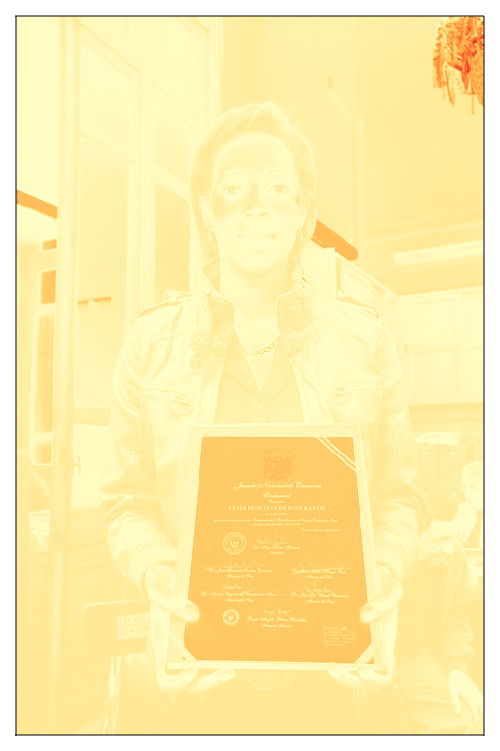
\includegraphics[width=\textwidth]{../figures/image2/image_02_distbg.png}
        \caption{Modelo de no piel, $\log(\text{Pr}(x | w=0))$.}
        % \label{fig:training_distbg}
    \end{subfigure}
    \hspace{0.25cm}
    %
    \begin{subfigure}[t]{0.2\textwidth}
        \centering
        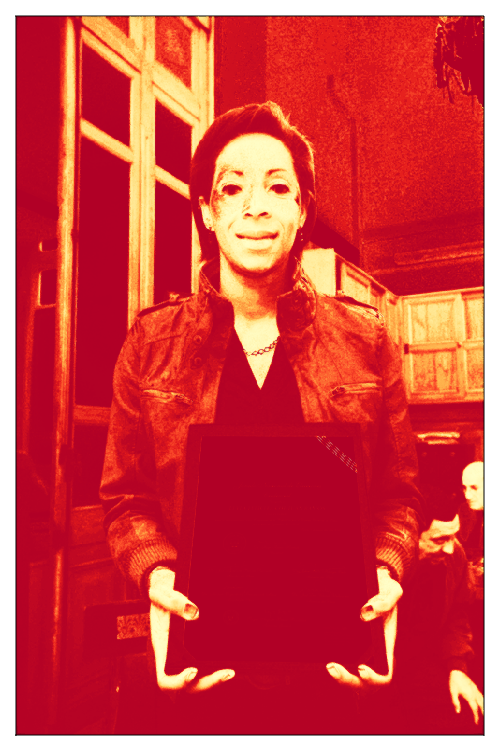
\includegraphics[width=\textwidth]{../figures/image2/image_02_postskin.png}
        \caption{Modelo a posteriori de piel, $\text{Pr}(w=1 | x^{\star})$.}
        % \label{fig:training_postskin}
    \end{subfigure}
    \hspace{0.25cm}
    %
    \begin{subfigure}[t]{0.2\textwidth}
        \centering
        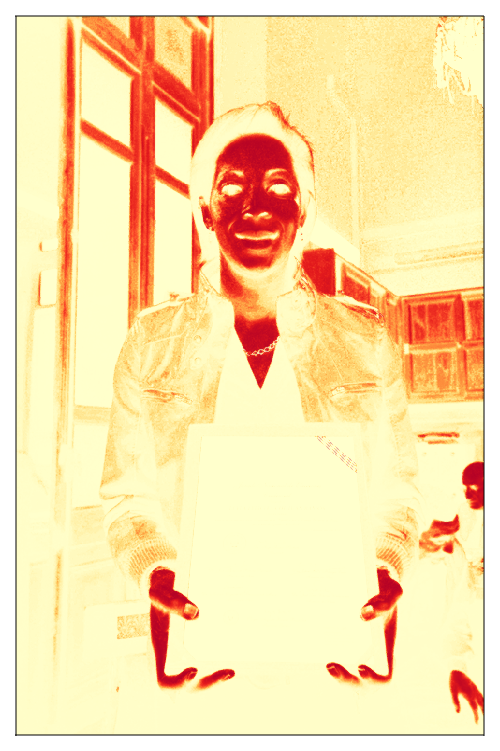
\includegraphics[width=\textwidth]{../figures/image2/image_02_postbg.png}
        \caption{Modelo a posteriori de no piel, $\text{Pr}(w=0 | x^{\star})$.}
        % \label{fig:training_postbg}
    \end{subfigure}
    %
    \begin{subfigure}[t]{0.2\textwidth}
        \centering
        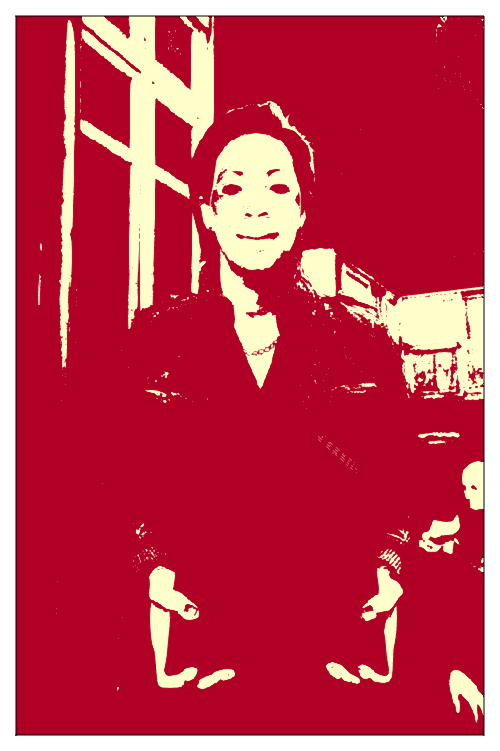
\includegraphics[width=\textwidth]{../figures/image2/image_02_treshskin_40percent.png}
        \caption{Piel; $\text{T} = 0.4$.}
        % \label{fig:training_treshskin_4}
    \end{subfigure}
    \hspace{0.25cm}
    %
    \begin{subfigure}[t]{0.2\textwidth}
        \centering
        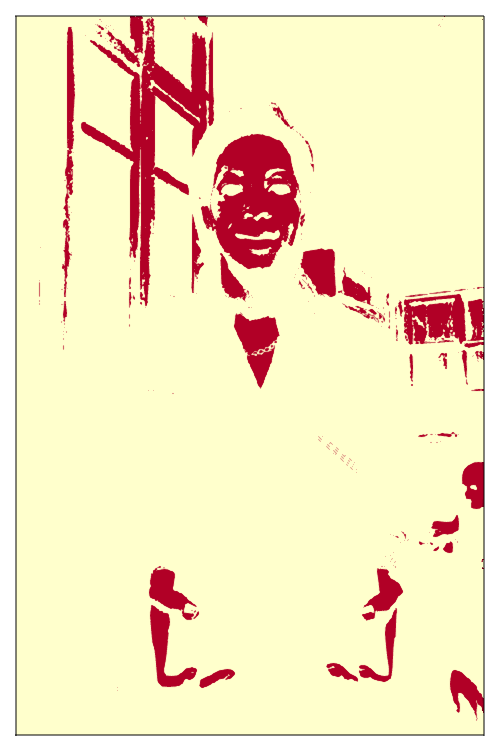
\includegraphics[width=\textwidth]{../figures/image2/image_02_treshbg_40percent.png}
        \caption{No piel; $\text{T} = 0.4$.}
        % \label{fig:training_treshbg_4}
    \end{subfigure}
    \hspace{0.25cm}
    %
    \begin{subfigure}[t]{0.2\textwidth}
        \centering
        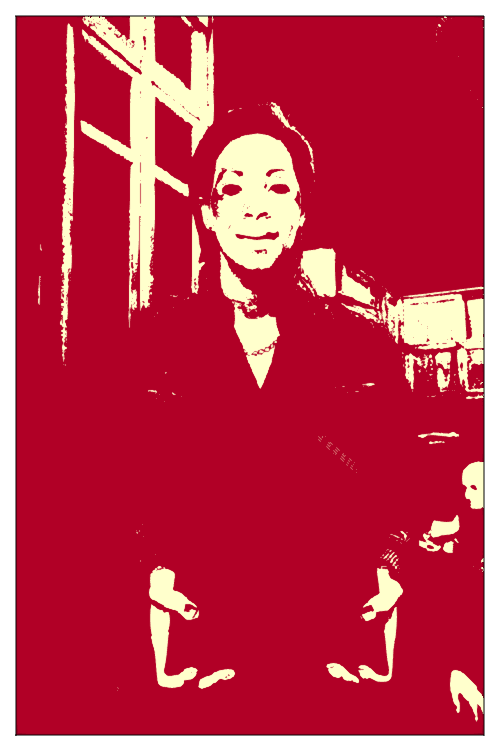
\includegraphics[width=\textwidth]{../figures/image2/image_02_treshskin_50percent.png}
        \caption{Piel; $\text{T} = 0.5$.}
        % \label{fig:training_treshskin_5}
    \end{subfigure}
    \hspace{0.25cm}
    %
    \begin{subfigure}[t]{0.2\textwidth}
        \centering
        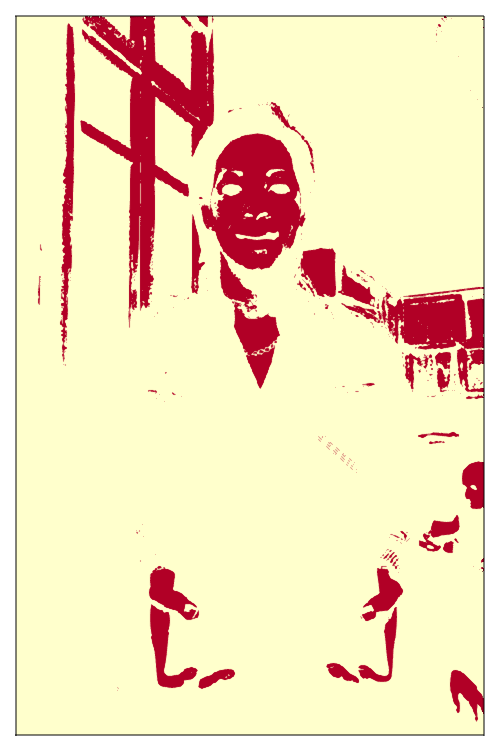
\includegraphics[width=\textwidth]{../figures/image2/image_02_treshbg_50percent.png}
        \caption{No piel; $\text{T} = 0.5$.}
        % \label{fig:training_treshbg_5}
    \end{subfigure}
    %
    \begin{subfigure}[t]{0.2\textwidth}
        \centering
        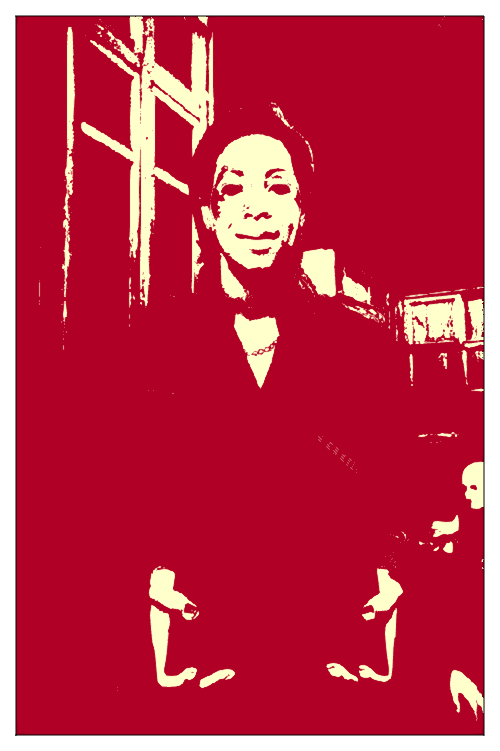
\includegraphics[width=\textwidth]{../figures/image2/image_02_treshskin_60percent.png}
        \caption{Piel; $\text{T} = 0.6$.}
        % \label{fig:training_treshskin_6}
    \end{subfigure}
    \hspace{0.25cm}
    %
    \begin{subfigure}[t]{0.2\textwidth}
        \centering
        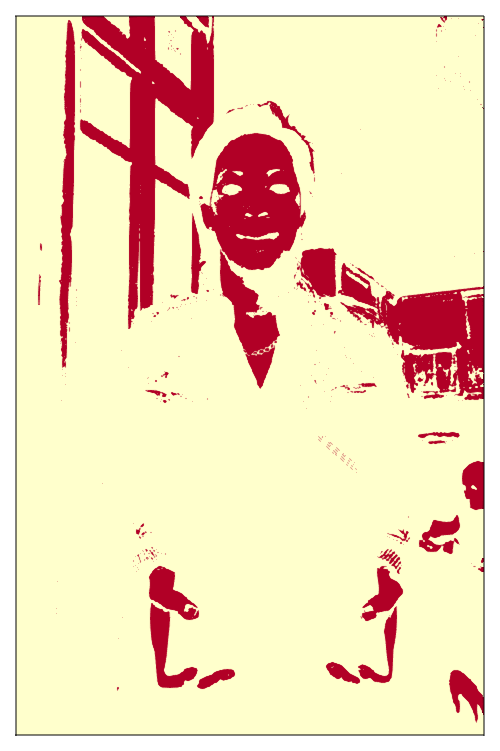
\includegraphics[width=\textwidth]{../figures/image2/image_02_treshbg_60percent.png}
        \caption{No piel; $\text{T} = 0.6$.}
        % \label{fig:training_treshbg_6}
    \end{subfigure}
    %
    \caption{Mapas de calor del modelo para piel y no piel de la imágen \cref{fig:imagen_prueba_no2}.}
    \label{fig:model_applied_no2}
\end{figure}


% \begin{minted}[
%     frame=none,
%     autogobble,
%     obeytabs=false,
%     breaklines,
%     tabsize=4,
%     linenos=true,
%     % numbersep=-10pt,
%     baselinestretch=1,
%     firstnumber=last,
%     bgcolor=bg!70,
%     ]{julia}
% \end{minted}

\clearpage
\section*{Apéndice}
\inputminted[
    frame=none,
    autogobble,
    obeytabs=false,
    breaklines,
    tabsize=4,
    linenos=true,
    % numbersep=-10pt,
    baselinestretch=1,
    firstnumber=1,
    bgcolor=bg!70,]{julia}{\codepath}

% https://github.com/NVlabs/ffhq-dataset

\nocite{*} % to call all references even if they are not cited in the text
\bibliography{references.bib}

\end{document}